\chapter{پژوهش‌های پیشین}\label{Chap:Chap2}
\minitoc
در این فصل بعد از بیان‌ مدل‌های مولد و دسته‌بند مورد استفاده در حوزه‌ی تولید دنباله، به بیان روش‌های پایه و مشکلات آن‌ها می‌پردازیم. سپس با بیان دقیق‌تر شبکه‌های مولد مقابله‌ای که بر اساس ایده‌ی آموزش مقابله‌ای هستند، روش‌های مبتنی بر یادگیری مقابله‌ای‌ را شرح می‌دهیم. روش‌های یادگیری مقابله‌ای را در چهار دسته درنظر می‌گیریم؛ این دسته‌بندی شامل روش‌های مبتنی بر
\lr{Gumbel Softmax}،
روش‌های مبتنی بر فضای ویژگی، روش‌های مبتنی بر یادگیری تقویتی و در آخر روش‌های با رویکرد تولید دنباله‌ی کلمات می‌شود. در پایان با جمع‌بندی این فصل را به اتمام می‌رسانیم.
\section{مقدمه}
بیشتر پژوهش‌های پیشین برای استفاده از شبکه‌های مولد مقابله‌ای در تولید دنباله به موضوع رفع مشکل انتقال گرادیان (که در بخش
\ref{Problem:GradientPass}
مورد بحث قرار گرفت) اختصاص داشته است. رویکرد‌های مختلفی برای این منظور وجود داشته است. 

برخی از روش‌ها به صورت تقریبی گرادیان انتقال یافته به مولد را به‌دست می‌آورند.
راه‌حل دیگر که رایج‌تر است، تبدیل مساله‌ی آموزش مولد به یک مساله‌ی یادگیری تقویتی است. این روش‌ها با تعیین پاداش برای مولد آموزش را انجام داده و گرادیان شبکه‌ی مولد را از این طریق محاسبه می‌کنند. در این دسته از پژوهش‌ها هدفی دیگر که دنبال می‌شود، افزایش اطلاعات موجود در پاداش  است. همچنین برخی از پژوهش‌ها سعی کرده اند با تغییر صورت مساله و تبدیل آن به مساله‌ای پیوسته، تولید دنباله را انجام دهند. در این فصل به هرکدام از این روشها پرداخته می‌شود.
در ادامه نماد گذاری معرفی شده که برای یک دست شدن بیشتر فصل در تمام فصل استفاده شده است.

 \subsection{نمادها }
در این بخش به بیان قرارداد‌ها و نماد‌هایی می‌پردازیم که در توضیح روش‌ها از این نمادگذاری استفاده شده است. این قراردادها و نمادگذاری‌ها در جدول
\ref{Table:SymbolsDefines}
مشخص شده است.

\begin{table}[!htb]
	\caption{جدول نماد‌ها}
	\label{Table:SymbolsDefines}
	\centering
	\begin{tabular}{|| c | r ||} 

		\hline
		\multicolumn{1}{||c|}{\bfseries نماد} & \multicolumn{1}{|c||}{\bfseries توضیحات} 
		\\ [0.5ex] 
		\hline\hline
		
		کلمه &
		کوچک‌ترین واحد دنباله کلمه است.
		\\ \hline
		$\mathcal{L}$  &
		برای نشان دادن تابع هزینه استفاده می‌شود که در صورت ذکر نکردن، آن را کمینه می‌کنیم.
		\\ \hline $L$  &
		طول دنباله‌ها یکسان فرض می‌شود و $L$ نشان دهنده‌ی طول دنباله‌ها است.
		\\ \hline $ٰV$  &
		\trans{اندازه‌ی واژگان}{Vocabulary Size}
		یعنی تعداد حالاتی که هر کلمه‌ی دنباله می‌تواند به خود بگیرد.
		\\ \hline $N$  &
		تعداد نمونه‌های آموزش 
		\\ \hline $ x^{(n)}$  &
		داده‌ی آموزش $n$ ام ($1 \leq n \leq N$)
		\\ \hline $x_l$  &
		کلمه‌ی $l$ از دنباله‌ی ‌$x$ ($1 \leq l \leq L$)
		\\ \hline $x_{a:b}$  &
		زیردنباله‌ی شامل کلمات $a$ ام تا $b$ ام ($1 \leq a < b \leq L$)
		\\ \hline $x_{:b}$  &
		زیردنباله‌ی شامل $b$ کلمه‌ی اول ($1 < b \leq L$)
		\\ \hline $P, P_{data}$  &
		نشان دهنده‌ی توزیع اصلی
		\\ \hline $p(x)$  &
		تابع چگالی توزیع اصلی
		\\ \hline $Q, P_{model}$  &
		نشان دهنده‌ی توزیع مدل است.
		\\ \hline $q(x)$  &
		تابع چگالی توزیع مدل
		\\ \hline $D_\phi(x)$  &
		نمایش تمیزدهنده به عنوان یک تابع است.
		\\ \hline $G_\theta$  &
		نشان دهنده‌ی شبکه‌ی مولد است.
		\\ \hline
	\end{tabular}
\end{table}

%\begin{itemize}
%	\item
%منظور از کلمه، کوچکترین واحد دنباله کلمه است.
%	\item
%از 
%$\mathcal{L}$
%برای نشان دادن تابع هزینه استفاده می‌شود که در صورت ذکر نکردن، آن را کمینه می‌کنیم.
%	\item $L$  :
%طول دنباله‌های یکسان فرض می‌شود و $L$ نشان دهنده‌ی طول دنباله‌ها است.
%	\item $ٰV$  :
%\trans{اندازه‌ی واژگان}{Vocabulary Size}
%یعنی تعداد حالاتی که هر کلمه‌ی دنباله می‌تواند به خود بگیرد
%	\item $N$  :
%تعداد نمونه‌های آموزش 
%	\item $ x^{(n)}$  :
%داده‌ی آموزش $n$ ام ($1 \leq n \leq N$)
%	\item $x_l$  :
%کلمه‌ی $l$ از دنباله‌ی ‌$x$ ($1 \leq l \leq L$)
%	\item $x_{a:b}$  :
%زیردنباله‌ی شامل کلمات $a$ ام تا $b$ ام ($1 \leq a < b \leq L$)
%	\item $x_{:b}$  :
%	زیردنباله‌ی شامل $b$ کلمه‌ی اول 	($1 < b \leq L$)
%		\item $P, P_{data}$  :
%نشان دهنده‌ی توزیع اصلی
%		\item $p(x)$  :
%تابع چگالی توزیع اصلی
%		\item $Q, P_{model}$  :	
%نشان دهنده‌ی توزیع مدل است
%		\item $q(x)$  :
%تابع چگالی توزیع مدل
%		\item $D_\phi(x)$  :	
%نمایش  تمیزدهنده به عنوان یک تابع است.
%		\item $G_\theta$  :	
%نشان دهنده‌ی شبکه مولد است.
%\end{itemize}
 \section{ مدل‌های مولد‌‌ }
 \label{Model:GenerativeModel:GeneralFormChainRule}
 در تمامی روش‌های ارائه‌شده، دنباله‌ها به صورت احتمالی توسط مدل مولد مدل‌سازی می‌شوند به طوری که توزیع احتمال دنباله به توزیع‌های ساده‌تری شکسته می‌شود که به صورت زیر است:
 \begin{equation}\label{Ch2:Equation:Prior:ChainRule}
 q(x;\theta) = q_1(x_1;\theta) \prod_{l=2}^{L}{q_l(x_l | x_{:l-1};\theta)}،
 \end{equation}
که این عبارت با کمک 
\trans{قاعده‌ی زنجیره‌ای}{Chain Rule}
به دست آمده است و توزیع احتمال دنباله به طول $L$ به توزیع‌های ساده‌تر تک متغیره $q_n(x_l | x_{:l-1};\theta)$ شکسته شده است.
 \newline
  لازم به ذکر است که هیچ استقلالی در  مدل‌سازی  به فرم گفته‌شده در رابطه‌ی \ref{Ch2:Equation:Prior:ChainRule} فرض نشده است و این موضوع باعث افزایش قابلیت مدل برای یادگیری توزیع‌های پیچیده و شامل ارتباطات طولانی در دنباله می‌شود \cite{Bowman2016VAE}.
\newline
 معمولا توزیع‌های $Q_l$   با استفاده از یک 
 \trans{شبکه‌ی عصبی بازگردنده}{Recurrent Neural Network}
 مدل می‌شود، ولی به تازگی شبکه‌های
  \trans{پیچشی}{Convolutional}
  نیز برای این منظور استفاده شده‌اند.
 \newline
  مدل‌های مولد را می‌توان به دو دسته تقسیم کرد:
   دسته‌ی اول مولد‌هایی هستند که با استفاده از نمونه‌گیری، دنباله‌های مختلف تولید می‌کنند. تمام قسمت تصادفی عملیات تولید نمونه در نمونه‌گیری خلاصه شده‌ است.
   دسته‌ی دوم مولد‌هایی هستند که برای تولید نمونه در یک فضای نهان، از یک توزیع ساده نمونه‌گیری کرده و سپس به کمک یک تابع تبدیل، این نمونه را‌ از فضای نهان به نمونه‌ی نهایی تبدیل می‌کنند.
%  ، در این روش کل قست تصادفی عملیات تولید نمونه در نمونه‌گیری از توزیع نهان است.
  دسته‌ی اول توزیع دنباله را به صورت صریح مدل می‌کنند، این در حالی است که توزیع در دسته‌ی دوم به شرط فضای نهان مدل می‌شود. در بخش‌های بعد به جزئیات مدل‌ها می‌پردازیم.
 \subsection{مدل‌ مولد بازگردنده مبتنی بر نمونه‌گیری}
 \label{Model:RecurrentSampling}
این مدل‌ها که از پراستفاده‌ترین مدل‌های مولد هستند، بر اساس رابطه‌ی
 \ref{Ch2:Equation:Prior:ChainRule}
 توزیع دنباله را با کمک یک ساختار بازگردنده مدل می‌کنند. ساختار
  \lr{LSTM}
  \cite{hochreiter1997LSTM}
  به عنوان یکی از انواع مرسوم شبکه‌های بازگردنده استفاده می‌شود.
 به صورت دقیق‌تر اگر در شبکه‌ی مورد استفاده اندازه‌ی
 \trans{ وضعیت مخفی}{Hidden State }
 برابر $h$ ، فضای نهان مورد استفاده برای کلمات $e$ و تعداد کلمات  $V$ باشد، علاوه بر شبکه‌ی بازگردنده دو ماتریس دیگر به پارامتر‌ها اضافه می‌شود. 
 ماتریس اول برای تبدیل کلمات به بردار ویژگی و دارای اندازه‌ی
$V\times e$
  است و سطر $l$-ام در آن شامل بردار ویژگی کلمه‌ی $l$-ام است.
 ماتریس دوم برای تبدیل وضعیت مخفی شبکه بازگردنده به توزیع روی کلمات است، اندازه این ماتریس
  $h\times V$
   است و با ضرب وضعیت مخفی در این ماتریس  برداری در اندازه‌ی کلمات به دست می‌آید. با اعمال تابع 
 \trans{بیشینه‌ی هموار}{Softmax}
 بر روی این بردار توزیع‌ای دسته‌ای 
 \LTRfootnote{Categorical}
 بر روی کلمات به دست می آید.
 \newline
 با وجود پراستفاده بودن این معماری، در پژوهشی جدید از نظر عملی  و تئوری نشان داده ‌شده است که این مدل‌های دارای محدودیت‌هایی  برای مدل کردن دنباله‌هایی مثل دنباله‌ی زبان طبیعی هستند
 \cite{yang2018breaking}.
 \temptext{میشه این بحث و ادامه داد و درمورد باتنلک حرف زد}
 \newline
 نمونه‌گیری از این مدل‌ها به این صورت است که در هر مرحله بخشی از دنباله‌ی تولید شده به مدل وارد می‌شود و مدل توزیعی برروی کلمه‌ی بعدی ایجاد می‌کند. کلمه‌ی بعدی دنباله با نمونه‌گیری از این توزیع، مشخص شده و این روال تکرار می‌شود. معمولا کلمه‌ای به عنوان کلمه‌ی «پایان» وجود دارد که هر زمان این کلمه تولید شود به معنی اتمام جمله است. در شکل
 \ref{Figure:GenrativeModel:Architecture:RecurrentSampling:Sampling}
 نحوه‌ی نمونه‌گیری از این مدل نمایش داده شده است.
 \begin{figure}[!htb]
 	{
 		\begin{center}
 			\subfigure[نمونه‌گیری از مدل]{\label{Figure:GenrativeModel:Architecture:RecurrentSampling:Sampling}\includegraphics[scale=0.7]{images/ArchitectureRNNGeneratorSampling.pdf}}
 			\hspace{1cm}
 			\subfigure[رویکرد حریصانه بیشینه‌گیری]{\label{Figure:GenrativeModel:Architecture:RecurrentSampling:Argmax}\includegraphics[scale=0.7]{images/ArchitectureRNNGeneratorArgmax.pdf}} 
 			\end{center}
 		\caption{مدل مولد بازگردنده مبتنی بر نمونه‌گیری}
 		\label{Figure:GenrativeModel:Architecture:RecurrentSampling:SamplingAndArgmax}
 	}
\end{figure}
 
 \subsubsection{سختی بیشینه گرفتن از مدل}
 از مشکلات مدل احتمالی تشریح شده، حالتی است که در گام آزمون به جای نمونه‌گیری به بیشینه‌گیری نیاز باشد، این مساله بیش‌تر در مدل‌های شرطی مطرح می‌شود.
 در این حالت یافتن نمونه با بیشترین احتمال بسیار هزینه‌بر است، زیرا پیچیدگی محاسباتی آن بر‌حسب تعداد عناصر دنباله، نمایی است.
 به همین دلیل رویکرد ساده‌ای مثل روش حریصانه مورد استفاده قرار گرفته و از  هر توزیع‌ $Q_n$ عنصر با بیشترین احتمال انتخاب می‌شود. در شکل
 \ref{Figure:GenrativeModel:Architecture:RecurrentSampling:Argmax}
 این روش نمایش داده شده است.
 می‌دانیم این نحوه‌ی نمونه‌گیری باعث انتخاب نمونه‌ها با احتمال کم‌تر از بیشینه می‌شود زیرا:
 \begin{equation}
 \prod_{l=1}^{L} \max_{\substack{x_l}} q_n(x_l | x_{1:l-1};\theta)
 \leq
 \max_{\substack{x}} \prod_{l=1}^{L} q_n(x_l | x_{1:l-1};\theta).
 \end{equation}
در روشی دیگر برای تقلیل این مشکل، به جای انتخاب یک لغت در هر مرحله، $k$ بهترین دنباله در هر مرحله انتخاب و نگهداری می‌شود که به این روش 
 \trans{جستجوی پرتویی}{Beam Search}
 گفته می‌شود
 \cite{bengio2015scheduled}  .
 
 \subsection{مدل‌های مولد مبتنی بر فضای نهان}
  \label{Model:Generative:Latent}
مدل‌های مولدی که دارای فضای نهان هستند، قابلیت مدل کردن صریح توزیع را از دست می‌دهند ولی در عوض امکان مشاهده و تغییر ویژگی‌های اصلی دنباله را به کمک فضای نهان دارند. به علاوه در روش‌های مثل 
\trans{خودرمزگذار وردشی}{Variational Autoencoder}،
 این مدل‌ها لازمه‌ی روش هستند
 \cite{Doersch16VAETut}.
\newline
در این مدل‌ها فرایند تولید نمونه به این صورت است که مقدار $z$ از فضای نهان نمونه گرفته می‌شود و مدل مولد به شرط $z$ نمونه را تولید می‌کند. این مدل‌ها بیش‌تر برای استفاده در شبکه‌های مولد مقابله‌ای در حوزه‌ی داده‌های پیوسته استفاده می‌شوند، ولی در حوزه‌ی داده‌های گسسته، استفاده از این مدل‌ها با مشکلاتی همراه است.
\newline
دو ساختار مطرح شده برای این مدل‌ها را در ادامه توضیح می‌دهیم.
 \subsubsection{ مدل‌ مولد بازگردنده مبتنی بر فضای نهان}
 \label{Model:Generative:Latent:RNN} 
این مدل‌ها ساختاری مشابه
\fullref{Model:RecurrentSampling}
دارند، با این تفاوت که متغیر نهان $z$ به مدل اضافه شده است. در ادامه دو نمونه از این مدل‌ها را توضیح می‌دهیم.
\newline
ساختاری که برای این شبکه‌ها در 
\cite{Bowman2016VAE}
پیشنهاد شده، با شکل
\ref{Figure:GenrativeModel:Architecture:RecurrentLatent:NonDet:Zfirst}
نشان داده شده است. تنها تفاوتی که این مدل با
\nameref{Model:RecurrentSampling}
دارد، در وضعیت مخفی اولیه‌ی شبکه است و وضعیت مخفی اولیه‌ی شبکه از مقدار نهان $z$ به دست می‌آید.
نوع دیگری از این ساختار در شکل
\ref{Figure:GenrativeModel:Architecture:RecurrentLatent:NonDet:Zall}
نمایش داده شده است که در آن علاوه بر وضعیت اولیه، متغیر نهان هم به عنوان ورودی به تمام مراحل شبکه‌ی بازگردنده وارد شده است. این ساختارها را مدل‌های غیرقطعی می‌نامیم، زیرا در این مدل‌ها با ثابت بودن مقدار $z$، تولید نمونه قطعیت نداشته و مجددا بعد از ورودی دادن $z$، فرایند تصادفی نمونه‌گیری در آن‌ها انجام می‌شود.
دو مدل غیرقطعی ارائه شده در پژوهش انجام شده در
\cite{Bowman2016VAE}
با روش خودرمزگذار وردشی آموزش دیده و برتری‌ای به هم دیگر ندارند. 
از نقد‌های وارد شده به مدل غیرقطعی این است که در آموزش تمایل به نادیده گرفتن مقدار نهان دارند
\cite{Yang2017ImprovedVAE, Bowman2016VAE}.
 \begin{figure}[!htb]
 	{
 		\begin{center}
 			\subfigure[]{\label{Figure:GenrativeModel:Architecture:RecurrentLatent:NonDet:Zfirst}\includegraphics[scale=0.7]{images/ArchitectureRNNLatentGeneratorSampling_1.pdf}}
 			\hspace{1cm}
 			\subfigure[]{\label{Figure:GenrativeModel:Architecture:RecurrentLatent:NonDet:Zall}\includegraphics[scale=0.7]{images/ArchitectureRNNLatentGeneratorSampling_2.pdf}} 
 		\end{center}
 	\caption{دو نمونه مدل بازگردنده‌ی مبتنی بر فضای نهان که به صورت غیرقطعی بعد از ورودی گرفتن نمونه را ایجاد می‌کنند.}
 		\label{Figure:GenrativeModel:Architecture:RecurrentLatent:NonDet:ZallAndZfirst}
 	}
 \end{figure}
 \newline
 در ساختار دیگری که برای مدل‌های بازگردنده‌ی مبتنی بر فضای نهان در
 \cite{Zhang2017TextGAN}
  پیشنهاد شده است، با مشخص شدن مقدار $z$، نمونه به صورت قطعی تولید شده و دیگر عملیات تصادفی در نمونه‌گیری وجود ندارد. 
  همان‌طور که این مدل در شکل 
  \ref{Figure:GenrativeModel:Architecture:RecurrentLatent:Det:Zall}
  نمایش داده شده است، متغیر نهان به تمام مراحل شبکه وارد می‌شود. نکته‌ای که در مورد این مدل وجود دارد این است که در عمل، مشتق‌ناپذیری
  $\argmax$
  باعث ایجاد مشکل در بعضی از روش‌های آموزش می‌شود. برای رفع این مشکل، عملیات $\argmax$ به وسیله‌ی تابع بیشینه‌ی هموار تخمین زده می‌شود. نحوه‌ی این تخمین در بخش
  \ref{Method:GumbelSoftmax:ArgmaxApprox}
  بیان خواهد شد.
  \begin{figure}[!htb]
  	\centering
  	\includegraphics[width=0.5\textwidth]{images/ArchitectureRNNLatentGeneratorArgmax.pdf} 
  	\caption{مدل بازگردنده‌ی مبتنی بر فضای نهان که به صورت قطعی بعد از ورودی گرفتن نمونه را ایجاد می‌کنند.}
  	\label{Figure:GenrativeModel:Architecture:RecurrentLatent:Det:Zall}
  \end{figure}
 
 \subsubsection{مدل‌ مولد پیچشی مبتنی بر فضای نهان}\label{Model:Generative:Latent:CNN}
نوع دیگری از مدل‌های مبتنی بر فضای داده در 
\cite{Yang2017ImprovedVAE}
استفاده شده است. این مدل رفتار غیرقطعی دارد و بعد از مشخص شدن مقدار نهان $z$، نمونه‌ی نهایی به صورت قطعی مشخص نیست. 
استفاده از
\trans{ شبکه‌ی عصبی پیچشی}{Convolutional Neural Networks}
به عنوان شبکه‌ی مولد، موضوع کمتر بررسی شده‌ای در حوزه‌ی تولید دنباله است. در ادامه به توضیح این ساختار می‌پردازیم.
\newline
شبکه‌ی پیچشی یک بعدی برای تولید دنباله مورد استفاده قرار می‌گیرد. در حالت عادی شبکه‌های پیچشی شرط 
\trans{علّی}{Causality}
بودن را ندارند؛ علّی بودن به این معنی است که بخشی از شبکه که کلمه‌ی $l$-ام را پیش‌بینی می‌کند، فقط تابع کلمات ورودی $1$ تا $l-1$ باشد. در گام آموزش، برای جلوگیری از رسیدن شبکه به حالت‌های نامطلوب نیازمند مدلی علّی هستیم، به همین دلیل شبکه‌ی پیچشی پیشنهاد شده، نوع علّی شبکه‌های پیچشی است.
\newline
به علاوه، برای افزایش 
\trans{اندازه‌ی میدان دریافتی}{Receptive Field Size}
از نوعی از شبکه‌های پیچشی به نام 
\trans{پیچشی متسع شده}{Dilated Convolution}
استفاده شده است.
شبکه‌ی پیچشی متسع شده در کنار افزایش اندازه‌ی میدان دریافتی، هزینه محاسباتی را زیاد نمی‌کند و به این صورت عمل می‌کند که اگر مقدار 
\trans{اتساع}{Dilation}
را
$d$
بنامیم، 
\trans{پیچش}{Convolution}
روی ورودی‌ها به صورتی اعمال می‌شود که ورودی‌ها
$d$
در‌میان در نظر گرفته می‌شود و
$d-1$
ورودی را در هر بخش در نظر نمی‌گیرد.  شبکه پیچشی معمولی را می‌توان حالت خاص شبکه‌ی پیچشی متسع‌شده با مقدار
$d=1$
در نظر گرفت
\cite{yu2015multi}.
در شکل 
\ref{Figure:GenrativeModel:Architecture:CNNLatent:Det:Zall}
این مدل برای حالت چهار ورودی  نمایش داده شده که در لایه‌ی اول  
$d=1$
و در لایه‌ی دوم
$d=2$
است. همان‌طور که در شکل مشخص است، مدل در تمام مراحل به مقدار نهان متصل است.
  \begin{figure}[!htb]
  	\centering
  	\includegraphics[width=0.5\textwidth]{images/ArchitectureImprovedVAEDecoder.pdf} 
  	\caption[ساختار شبکه‌ی رمزگشای پیچشی متسع شده ]
  	{ساختار شبکه‌ی رمزگشای پیچشی متسع شده برای چهار ورودی
	  		 \cite{Yang2017ImprovedVAE}
  		 }
  	\label{Figure:GenrativeModel:Architecture:CNNLatent:Det:Zall}
  \end{figure}
  \temptext{جزئیات مثل مشترک بودن وزن، اینکه امبد می‌کنیم و ...}
  
 \section{مدل‌های دسته‌بند }\label{Model:Classifier}
مدل‌های دسته‌بند دو دسته‌ای در روش‌های مبتنی بر یادگیری مقابله‌ای مورد استفاده هستند. این شبکه‌ها دنباله را  به عنوان ورودی گرفته و عددی بین صفر و یک را خروجی می‌دهد. دو نوع شبکه‌ی پرکاربرد برای این منظور وجود دارد که در ادامه معرفی شده‌اند.
 \subsection{مدل‌ دسته‌بند بازگردنده}\label{Model:Classifier:RNN}
این مدل‌ها یک شبکه‌ی بازگردنده که معمولا
\lr{LSTM}
است، استفاده کرده و بعد از بردن کلمات دنباله به فضای ویژگی، این دنباله‌ی ویژگی‌ها را به مدل بازگردنده وارد کرده و در نهایت برای ساختن مقدار خروجی، تبدیلی خطی بر روی آخرین وضعیت مخفی در نظر گرفته و با اعمال تابع فعال‌ساز سیگموید خروجی بین صفر و یک ایجاد می‌کنند.
 \subsection{مدل‌ دسته‌بند پیچشی}\label{Model:Classifier:CNN}
روش دیگر دسته‌بندی، مبتنی بر استفاده از شبکه‌های پیچشی یک بعدی است.
همان‌طور که در شکل
\ref{Figure:DiscriminatorModel:Architecture:CNN}
نمایش داده شده است، این شبکه‌ها در ابتدا کلمات دنباله را به فضای ویژگی برده و سپس به‌وسیله‌ی اعمال پیچش‌هایی با  فیلترهای با
اندازه‌های مختلف، از دنباله ویژگی استخراج می‌کنند. این ویژگی‌ها با طول دنباله رابطه داشته و  اندازه‌ی ثابتی ندارند، از این رو در طول دنباله بر روی این ویژگی‌ها با بیشینه‌گیری 
\trans{رای‌گیری}{Pooling}
انجام می‌شود و  در نهایت به تعداد فیلترها از دنباله ویژگی استخراج می‌شود. در گام نهایی با یک یا چند لایه‌ی
\trans{تمام‌متصل}{Fully Connected}،
 این ویژگی‌ها به یک عدد تبدیل شده که به عنوان خروجی دسته‌بند استفاده می‌شود
\cite{Yoon14CNNClassifier}.
\newline
به بیان ساده‌تر این مدل ویژگی‌هایی را از 
\trans{\ngram}{n-gram}های
دنباله استخراج می‌کند و مستقل از جایی که این
\ngram{}ها
قرار دارند، از روی این ویژگی‌ها خروجی نهایی را پیش‌بینی می‌کند.
  \begin{figure}[!htb]
  	\centering
  	\includegraphics[width=0.7\textwidth]{images/ArchitectureCNNDiscriminator.pdf} 
  	\caption[ساختار شبکه‌ی پیچشی یک بعدی به عنوان دسته‌بند]
  	{ساختار شبکه‌ی پیچشی یک بعدی به عنوان دسته‌بند 
  		\cite{Zhang2017TextGAN}
  		}
  	\label{Figure:DiscriminatorModel:Architecture:CNN}
  \end{figure}

 \section{یادگیری مبتنی بر بیشینه درست‌نمایی}
 بیشینه کردن درست‌نمایی از قدیم جزء روش‌های پراستفاده بوده است. در این بخش بعد از توضیحات اولیه  به بررسی روش‌هایی که تابع هزینه‌ی مبتنی بر بیشینه درست‌نمایی دارند، می‌پردازیم. در ابتدا روش
   \trans{جبر معلم}{Teacher Forcing}
که روش پایه‌ی تولید دنباله محسوب می‌شود، توضیح داده، سپس به بیان مشکل  اُریبی مواجهه  پرداخته و راه‌کار ارائه شده برای رفع آن را بررسی می‌کنیم. در انتها به بررسی روش‌های خودرمزگذار وردشی می‌پردازیم، که هدفشان علاوه بر تولید دنباله یافتن نمایشی در فضای نهان برای دنباله‌ها است.
 \newline
در روش بیشینه کردن  درست نمایی مدلی پارامتری برای تخمین توزیع احتمال ارائه می‌شود، که $\theta$ پارامتر آن است. درست‌نمایی مدل به ازای پارامتر $\theta$ برابر 
 $\prod_{n=1}^{N}P_{model}(x^{(n)};\theta)$
 است، که  $x^{(i)}$ها داده‌های آموزش هستند.
 اصل بیشینه درست‌نمایی به سادگی می‌گوید که باید پارامتر $\theta$ به صورتی انتخاب شود که درست‌نمایی بیشینه
 شود \cite{goodfellow2016nips}.
 \newline
 به بیانی دیگر بیشینه کردن درست‌نمایی هم‌ارز کم کردن فاصله‌ی 
\lr{Kullback-Leibler  (KL)}
 بین توزیع داده‌های واقعی و توزیع مدل است:
 \begin{equation}
 \theta^\star = \arg \max_{\substack{\theta}} D_{KL}(P_{data}(x) || P_{model}(x;\theta)) ,
 \end{equation}
 که در عمل به $P_{data}(x)$ دسترسی نداشته و فقط $N$ نمونه از این توزیع داریم، و به همین دلیل به جای استفاده از $P_{data}(x)$ از تقریب $\hat{P}_{data}(x)$  استفاده می‌کنیم.
 $\hat{P}_{data}(x)$
  یک توزیع تجربی است که چگالی احتمال فقط روی $N$ نمونه‌ وجود دارد. کمینه کردن فاصله‌ی KL بین 
 $\hat{P}_{data}(x)$
 و 
 $P_{model}$
 معادل بیشینه درست‌نمایی روی داده‌های آموزش است \cite{goodfellow2016nips}.
 \subsection{روش  جبر معلم}\label{sec2:exposurebias}
  \label{Method:TeacherForcing}
 روش جبر معلم پایه‌ای‌ترین راه برای آموزش توزیع دنباله و تولید دنباله‌های جدید است.
 در روش  جبر معلم تابع هزینه‌ براساس بیشینه درست‌نمایی است و  معمولا 
 \fullref{Model:RecurrentSampling}
 به عنوان مولد استفاده می‌شود. بنابراین تابع هزینه از رابطه‌
\ref{Ch2:Equation:Prior:ChainRule}
به صورت زیر  به دست می‌آید:
\begin{equation}
\mathcal{L} = \sum_{n=1}^N \sum_{l=1}^{L} \log Q_l(x_l^{(n)}|x_{1:n-1}^{(n)})
\end{equation}
این  تابع هزینه نشان می‌دهد که برای آموزش،  زیر دنباله‌ی 
$x_{:n}$
به مدل وارد می‌شود و انتظار می‌رود که مدل کلمه‌ی 
$x_{n+1}$
را پیش‌بینی کند. در شکل
\ref{Figure:TeacherForcing:ExposureBias:Train}
روال آموزش نشان داده شده است.
 \begin{figure}[!htb]
 	{
 		\begin{center}
 			\subfigure[مرحله‌ی آموزش]{\label{Figure:TeacherForcing:ExposureBias:Train}\includegraphics[scale=1.2]{images/ExposureBias_Train.pdf}}
 			\hspace{1cm}
 			\subfigure[مرحله‌ی آزمون]{\label{Figure:TeacherForcing:ExposureBias:Test}\includegraphics[scale=1.2]{images/ExposureBias_Test.pdf}} 
 		\end{center}
 		\caption[روش  جبر معلم در دو فاز آموزش و آزمون]
 		{روش  جبر معلم در دو فاز آموزش و آزمون \cite{lamb2016professor}}
 		\label{Figure:TeacherForcing:ExposureBias}
 	}
 \end{figure}
  \subsubsection{اُریبی مواجهه}
  همان‌طور که توضیح داده شد، در آموزش روش جبر معلم فقط داده‌های آموزش وارد شبکه می‌شود، بنابراین شبکه به شرط زیر دنباله‌های واقعی و درست، آموزش دیده تا بتواند کلمه‌ی بعدی را پیش‌بینی کند.
ولی در فاز آزمون که از شبکه‌ی آموزش‌دیده نمونه‌گیری می‌کنیم، داده‌های واقعی را نداریم که از آن به عنوان ورودی مدل استفاده شود و راه‌حلی که وجود دارد ورودی دادن دنباله‌ی تولید شده توسط خود مدل است. نحوه‌ی تولید نمونه‌ها در فاز آزمون در شکل
\ref{Figure:TeacherForcing:ExposureBias:Test}
 نمایش داده شده است.
 بنابراین توزیع ورودی که بر‌حسب آن مدل آموزش دیده در فاز آزمون تغییر کرده است و این تغییر ورودی موجب خطا در خروجی پیش‌بینی شده می‌شود. این خطا به صورت تجمعی در طول دنباله بیشتر شده و باعث کاهش  کیفیت نمونه‌های تولیدی می‌شود
 \cite{SeqGAN, Huszar15HowNot, bengio2015scheduled}
 . این رفتار باعث تولید دنباله‌هایی می‌شود که دارای کلمات مناسب و با کیفیتی در ابتدای دنباله  هستند، اما در کلمات جلوتر کیفیت کاهش می‌یابد
 \cite{Zhang2017TextGAN}.
 
 از آنجا که در گام آموزش شبکه فقط در مواجهه داده‌های کاملا درست قرار گرفته و در آزمون در مواجهه داده‌های تولید شده قرارگرفته، این مشکل  اُریبی مواجهه نامیده  می‌شود
  \cite{bengio2015scheduled, press2017langwasserstein}.

 \subsection{روش  نمونه برداری زمان‌بندی شده}
 برای حل مشکل اُریبی مواجهه در مقاله‌ی
  \cite{bengio2015scheduled}
 راه‌کاری به نام 
 \trans{ نمونه‌برداری زمان‌بندی شده }{Scheduled Sampling}
 پیشنهاد شده است که در عمل باعث بهبود می‌شود ولی  دارای مشکلاتی است که در ادامه بعد از معرفی روش، به آن می‌پردازیم. این روش  هم‌چنین به نام
 \trans{داده به عنوان اثبات‌گر}{Data As Demonstrator (DAD)}
 شناخته می‌شود
 \cite{ranzato2015sequence}.
 \newline
 همانطور که در بخش
 \ref{Method:TeacherForcing}
 توضیح داده شد، مشکل اُریبی مواجهه ریشه در تفاوت پیکربندی شبکه بین دو فاز آموزش  و آزمون دارد؛
 روش
  \trans{ جبر استاد}{Professor Forcing}
   برای حل این مشکل، در گام‌های آموزش نیز بعضی از عناصر دنباله ورودی به شبکه را از داده‌های مصنوعی و تولید شده توسط خود شبکه انتخاب می‌کند.
 \newline
 برای ساخت دنباله‌ی ورودی در مرحله‌ی آموزش، به ازای هر کلمه با احتمال $\epsilon$ از داده‌های واقعی استفاده شده و با احتمال 
 $1-\epsilon$
 از کلمه نمونه‌گیری شده از خود مدل استفاده می‌شود. پارامتر $\epsilon$ در ابتدای آموزش مقدار برابر یک دارد و این مقدار به تدریج کاهش پیدا می‌کند تا به صفر برسد. با این کار مدل به تدریج برای تولید دنباله در ادامه‌ی نمونه‌های تولید شده از خودش در زمان آزمون آماده می‌شود.
 این روال در شکل 
 \ref{Figure:ScheduledSampling:Architecture}
 نمایش داده شده است.
\begin{figure}[!htb]
	\centering
	\includegraphics[width=0.8\textwidth]{images/ArchitectureSS.png} 
	\caption[نمای کلی روش نمونه‌برداری زمان‌بندی شده]
	{
نمای کلی روش نمونه‌برداری زمان‌بندی شده، انتخاب هر عنصر دنباله مشابه پرتاب یک سکه است که تصمیم بگیریم از نمونه‌ی تولید شده توسط مدل و یا نمونه‌ی با مقدار واقعی استفاده کنیم
		\cite{bengio2015scheduled}.
	}
	\label{Figure:ScheduledSampling:Architecture}
\end{figure}
\newline
مشکلات این روش به شرح زیر است:
\begin{itemize}
	\item 
در این روش در هر جایگاه از دنباله، مستقل از دنباله‌ی تولید شده تا آن کلمه، مقدار هدف برای کلمه‌ی بعدی  (یعنی مقداری که می‌خواهیم بیشترین احتمال را در خروجی داشته باشد) برابر مقداری است که داده واقعی در جایگاه متناظر دارد. این رفتار ممکن است در بعضی حالات باعث سوق دادن مدل به پیش‌بینی اشتباه شود
	 \cite{ranzato2015sequence}.
	 \newline
	 برای مثال فرض کنید دنباله‌ی واقعی جمله‌ی «من یک پیاده‌روی طولانی داشتم» باشد. 
	 در آموزش با عملیات تصادفی که در روش وجود دارد سه کلمه‌ی اول ورودی از داده‌ی واقعی انتخاب شده و کلمه آخر توسط مدل تولید شود. پیشوند تولید شده در این حالت  می‌تواند برابر «من یک پیاده‌روی داشتم» شود (کلمه‌ی آخر توسط مدل پیش‌بینی شده است). در این شرایط در آموزش مدل را به سمتی می‌بریم که کلمه‌ی بعدی از داده‌ی اصلی یعنی کلمه «داشتم» را پیش‌بینی کند، به بیان دیگر مدل را به سمتی سوق می‌دهیم که در کل عبارت «من یک پیاده‌روی داشتم داشتم» را تولید کند.
	 \item
به صورت تئوری در
	  \cite{Huszar15HowNot}
	  بررسی شده است که این روش تخمین‌گر صحیحی برای بیشینه درست‌نمایی نیست، یعنی اگر ظرفیت مدل و تعداد داده‌های آموزش به بی‌نهایت میل کند، مدل آموزش دیده به سمت مدل با بیشینه درست‌نمایی نمی‌رود و تخمین‌گر
	  \trans{اُریبی}{Bias}
دارد.
	   \temptext{میشه محاسبات تئوری اثبات را وارد کرد}
\end{itemize}
 
 \subsection{روش‌های مبتنی بر خودرمزگذار وردشی}
 روش‌هایی مبتنی بر خودرمزگذار وردشی  در کاربرد تولید دنباله بیش‌تر به این منظور توسعه یافته‌اند که علاوه بر تولید دنباله، فضای نهان برای دنباله‌ها تولید کنند که در آن فضا، مفاهیم اساسی دنباله بیان شود.
 مثلا در زبان طبیعی موضوع جمله و یا ویژگی‌های معنایی آن از جمله مفاهیمی هستند که در فضان نهان به دنبال آن هستیم. حالت موفق این نمایش در فضای نهان می‌تواند به این صورت باشد که بین نمایش دنباله‌ها بتوان روابط جمع و تفریق به دست آورد، مثلا بتوان در فضای نهان دنباله‌های زبان طبیعی برداری پیدا کرد که با اضافه کردن آن به یک جمله، با حفظ مفهوم، آن را به سمت غیر رسمی‌تر شدن ببرد و یا با تفریق آن متن را به سمت رسمی‌تر شدن ببرد. برای این هدف مدل ارائه شده در بخش \ref{Model:RecurrentSampling} مناسب نیستند زیرا فضای نهانی ندارند و ویژگی‌هایی  هم که در هر گام این روش‌ها به دست می‌آید، به هدف تولید کلمه‌ی بعدی است و نه برای دربرداشتن مفاهیم دنباله
  \cite{Bowman2016VAE}.
برای به دست آوردن فضای نهان می‌توان از روش خودرمزگذار وردشی استفاده کرد. به عبارت دیگر این روش‌ها راهی برای یادگیری در مدل‌های معرفی‌شده در بخش \ref{Model:Generative:Latent:RNN} هستند.
 \newline
روش خودرمزگذار وردشی شامل دو شبکه‌ی 
 \trans{ رمزگذار}{Encoder}
و
 \trans{رمزگشا}{Decoder}
است و تابع هزینه‌ی آن کران پایینی برای درست‌نمایی است که با بیشینه کردن این کران سعی در بیشینه کردن درست نمایی داریم، این کران به صورت زیر است
\cite{Doersch16VAETut, Bowman2016VAE}:
\begin{equation}\label{Ch2:Equation:VAE:LowerBound}
\mathfrak{L}(\theta;x)=-\mathfrak{D}_{KL}(q_{\theta}(z|x) \Vert p(z))
+
\ME_{q_{\theta}(z|x)}[\log p_{\theta}(x|z)].
%\leq log p(x)
\end{equation}
در رابطه‌ی
\ref{Ch2:Equation:VAE:LowerBound}
توزیع
$q_{\theta}(z|x)$
مدل احتمالی رمزگذار،
$p_{\theta}(x|z)$
مدل احتمالی رمزگشا است و
$p(z)$
توزیع احتمالی است که فرض کرده‌ایم متغیر نهان
$z$
از آن می‌آید؛ سمت راست رابطه‌ی 
\ref{Ch2:Equation:VAE:LowerBound}
شامل دو عبارت می‌شود. اولی عبارتی بر حسب فاصله‌ی 
\lr{KL}
است که توزیع
\trans{پسین}{Posterior}
 یعنی $q(z|x)$
را به توزیع
\trans{پیشین}{Prior}
 یعنی $p(z)$
نزدیک می‌کند. عبارت دوم را
\trans{تابع هزینه‌ی بازسازی}{Reconstruction Loss}
 می‌نامیم و سعی دارد شبکه را به این سمت سوق دهد که ورودی را در خروجی تولید کند. معمولا توزیع پیشین و پسین گاوسی فرض می‌شود، توزیع پیشین گاوسی با میانگین صفر و کواریانس همانی است و توزیع پسین با گاوسی  با کواریانس قطری است که پارامتر‌های آن توسط شبکه بر حسب ورودی مشخص می‌شود. لازم به ذکر است که در حالتی که توزیع پسین و پیشین گاوسی است، برای فاصله‌ی
 \lr{KL}
 در رابطه‌ی
 \ref{Ch2:Equation:VAE:LowerBound}
 فرم بسته وجود دارد
 \cite{Doersch16VAETut, Bowman2016VAE}.
\newline
در مقاله‌های
\cite{Bowman2016VAE}
و
\cite{Yang2017ImprovedVAE}
دو نمونه استفاده از خودرمزگذار وردشی در حوزه‌ی دنباله ‌پیشنهاد شده است، هر دوی این روش‌ها شبکه‌ی رمزگذاری  از نوع
  \lr{LSTM}
  دارند ولی  در  روش اول شبکه‌ی رمزگشا
  \lr{LSTM}
  و در روش دوم شبکه‌ای پیچشی است، در ادامه به این دو روش می‌پردازیم.
\subsubsection{شبکه‌ی \lr{LSTM} به عنوان رمزگشا}
همان‌طور که گفته شد روش ارائه شده در
  \cite{Bowman2016VAE}
برای رمزگذار  و رمزگشا از شبکه‌ی
\lr{LSTM}
استفاده کرده است، این روش را در ادامه
\lr{VAE-LSTM-LSTM}
می‌نامیم.
\newline
روش 
\lr{VAE-LSTM-LSTM}
همان‌طور که گفته شد رمزگذار و رمزگشا از نوع 
\lr{LSTM}
دارد.
شبکه رمزگذار به وسیله‌ی تبدیلی خطی بر روی آخرین وضعیت مخفی شبکه‌ی بازگردنده، پارامترهای توزیع پسین را محاسبه می‌کند.
هم‌چنین از
\fullref{Model:Generative:Latent:RNN}
در حالت غیرقطعی، به عنوان شبکه‌ی رمزگشا استفاده شده است.
 ساختار توضیح داده شده در شکل
 \ref{Figure:VAE:Architecture}
 برای یک نمونه داده‌ی ورودی بیان شده است.
\begin{figure}[!htb]
	\centering
	\includegraphics[width=0.8\textwidth]{images/ArchitectureVAE.pdf} 
	\caption[نمای کلی شبکه‌ی خودرمزگذار وردشی با رمزگذار و رمزگشای
	\lr{LSTM}
	برای یک نمونه ورودی]
	{
		نمای کلی شبکه‌ی خودرمزگذار وردشی با رمزگذار و رمزگشای
		\lr{LSTM}
		برای یک نمونه ورودی
		\cite{Bowman2016VAE}
	}
	\label{Figure:VAE:Architecture}
\end{figure}
 \newline
در حالت عادی مدلی که اطلاعات مفید رمزگذار را در 
 $z$
 ذخیره می‌کند، دارای مقدار غیر صفر برای جمله‌ی فاصله‌ی KL در رابطه‌ی 
\ref{Ch2:Equation:VAE:LowerBound}
 است، یعنی دو توزیع پسین و پیشین  دقیقا برابر نمی‌شود. 
 ولی در عمل زمانی که شبکه‌ی
 \lr{VAE-LSTM-LSTM}
 با روش معمول آموزش شبکه‌های خودرمزگذار وردشی آموزش داده می‌شود، در بیش‌تر موارد این رفتار دیده شده و مقدار KL صفر می‌شود که به این معنی است که دو توزیع
 $p(z)$
 و
 $q_{\theta}(z|x)$
 یکسان می‌شوند. زمانی که مدل این رفتار را بروز می‌دهد، می‌تواند هر توزیع دلخواهی را به عنوان خروجی مستقل از
 $z$
 تولید کرده و مشابه روش جبر معلم عمل کند 
 \cite{Bowman2016VAE}.
   دلیل این رفتار کاملا مشخص نیست ولی  ساختار
   \lr{LSTM}
   استفاده شده به عنوان  رمزگشا این خاصیت را دارد که اطلاعات ورودی رمزشده از رمزگذار را نادیده می‌گیرد
   \cite{Yang2017ImprovedVAE, Bowman2016VAE}.
 \newline
 در
 \lr{VAE-LSTM-LSTM}
 دو راهکار برای رفع مشکل صفر شدن
  \lr{KL}
  پیشنهاد شده است:
  \begin{itemize}
  	\item 
با وزن‌دار کردن جمله‌ی 
  	\lr{KL}
  	در رابطه‌ی
  	\ref{Ch2:Equation:VAE:LowerBound}، 
  به طوری که این وزن در ابتدا صفر باشد تا این موضوع باعث شود مدل بدون مشکلی در افزایش تابع هزینه، اطلاعات رمزگذار را در
  	$\vec{z}$
  	رمز کند و خطای بازسازی کمتر شود. سپس در ادامه‌ی آموزش، این وزن افزایش یافته تا هدف دیگر آموزش که نزدیک کردن دو توزیع 
  	$p(z)$
  	و
  	$q_{\theta}(z|x)$
  	به هم است، برآورده شود. 
  	\item
با جایگذاری بعضی از کلمات ورودی، شبکه رمزگشا به سمتی سوق داده می‌شود که به متغیر نهان اهمیت بیشتری دهد. در این جایگذاری کلمات ورودی به صورت تصادفی به کلمه‌ی 
  	\lr{UNK}
  	(به معنی نامعلوم)
تبدیل می‌شوند. بنابراین رمزگشا مجبور شود به سمتی برود که اطلاعات حذف شده را از متغیر نهان استخراج کند و به متغیر نهان اهمیت بیشتری دهد
  	\cite{Bowman2016VAE}.
  \end{itemize}
 نتایج این روش با وجود به دست آوردن نمایش مخفی از دنباله، در تولید دنباله‌ی زبانی ضعیف‌تر از مدل‌های ساده‌ی زبانی مثل روش جبر معلم بوده است
  \cite{Bowman2016VAE}؛
یکی از دلایلی که برای ضعف این روش ذکر می‌شود این است که توزیع پسینی که شبکه‌ی رمزگذار می‌سازد، کل فضای نهان را پوشش نمی‌دهد و بخش زیادی از این فضا به دنباله‌ی معتبری متناظر نمی‌شود
   \cite{Zhang2017TextGAN}.

\subsubsection{شبکه‌ی پیچشی به عنوان رمزگشا}
در راهکاری دیگر که در 
 \cite{Yang2017ImprovedVAE}
 ارائه شده، با جایگذاری 
 \ref{Model:Generative:Latent:CNN}
به صورت غیرقطعی به عنوان رمزگشا، نتایج بهبود داده شده است. نمای کلی شبکه در شکل
 \ref{Figure:ImprovedVAE:Architecture}
 نشان داده شده است، این روش را
 \lr{VAE-LSTM-CNN}
 می‌نامیم. با ساختار جدید علاوه بر بهبود روش نسبت به مدل 
  \lr{VAE-LSTM-LSTM}،
نتایج در حوزه‌ی تولید دنباله نسبت به روش‌ پایه‌ی جبر معلم هم بهبود یافته است.
 \newline
   \temptext{جزئیات و بررسی‌ها دیگه داره کارشون}
 \begin{figure}[!htb]
 	\centering
 	\includegraphics[width=0.65\textwidth]{images/ArchitectureImprovedVAE.pdf} 
 	\caption[ساختار کلی شبکه‌ی خودرمزگذار وردشی با رمزگذار \lr{LSTM} و رمزگشای پیچشی]
 	{ساختار کلی شبکه‌ی خودرمزگذار وردشی با رمزگذار ‎\lr{LSTM} و رمزگشای پیچشی 
 		\cite{Yang2017ImprovedVAE}
 		}
 	\label{Figure:ImprovedVAE:Architecture}
 \end{figure}

 \section{شبکه‌های مولد مقابله‌ای}
  \label{Method:GAN:Deep}
 در بخش
 \ref{Method:GAN:Shalow}
 به بیان مختصری از شبکه‌های مولد مقابله‌ای پرداختیم، در این بخش به صورت دقیق‌تر به این موضوع می‌پردازیم.
لازم به ذکر است که منظور از یادگیری مقابله‌ای اید‌ه‌ای مشابه با پژوهش شبکه‌های مولد مقابله‌ای
 \cite{Goodfellow2014}
 است.
 \newline
اساس کار شبکه‌های مولد مقابله‌ای
 \cite{Goodfellow2014}
 بازی بین دو شبکه است؛ شبکه‌ی اول مولد است که نمونه‌‌ تولید می‌کند و شبکه‌ی دوم یک دسته‌بند  احتمالاتی  و دو دسته‌ای است که بر روی نمونه‌های تولید شده و واقعی قضاوت کرده و با این قضاوت شبکه‌ی مولد را به سمت بهبود راهنمایی می‌کند. به صورت دقیق‌تر، شبکه‌ی مولد به سمتی می‌رود که دسته‌بند را به خطا بیاندازد و دسته‌بند هم به سمتی می‌رود که دسته‌بندی درست انجام دهد؛ یک حالت تعادل این بازی زمانی است که مولد نمونه‌های مشابه نمونه‌های واقعی تولید کند و دسته‌بند هم برای داده‌های واقعی و هم برای داده‌های تولید شده احتمال $\frac{1}{2}$ نسبت دهد. زیرا در حالتی که دو دسته‌ی داده دارای توزیع یکسان هستند، تشخیص درست برای دسته‌بند دادن احتمال $\frac{1}{2}$ است.
 \newline
  مدل مولد در این روش، در واقع یک تابع تبدیل است که تبدیلی از فضای نهان به فضای نمونه‌ها انجام می‌دهد. فضای نهان توزیع ساده‌ای مثل گاوسی در نظر گرفته می‌شود. بنابراین روال تولید نمونه به این صورت می‌شود که بعد از نمونه‌گیری از توزیع گاوسی، شبکه‌ی مولد بر روی این نمونه اعمال شده و نمونه‌ی نهایی تولید می‌گردد.
  مدل دسته‌بند که به نام تمیزدهنده  شناخته می‌شود، یک شبکه‌ی دسته‌بند دو دسته‌ای عادی است.
  در شکل
  \ref{Figure:GAN:Architecture}
  نمایی از یادگیری مقابله‌ای نمایش داده شده است.
  \begin{figure}[!htb]
  	\centering
  	\includegraphics[width=1\textwidth]{images/ArchitectureGAN.png} 
  	\caption{نمای کلی روش یادگیری مقابله‌ای}
  	\label{Figure:GAN:Architecture}
  \end{figure}
  \newline
  تابع هزینه‌‌ی این روش به صورت زیر است:
  \begin{equation}\label{Ch2:Equation:GAN:MinMaxObjective}
  \min_G \max_D V(D, G) = \ME_{x \sim P_{data}} [log D(x)] + \ME_{z \sim P_z} [log(1-D(G(z)))].
  \end{equation}
  در رابطه‌ی
  \ref{Ch2:Equation:GAN:MinMaxObjective}
  عبارت سمت راست، منفی تابع هدف دسته‌بندی بین مجموعه داده‌های 
  $\{x | x \sim P_{data}\}$
  به عنوان دسته‌ی با برچسب صفر
  و مجموعه داده‌ی
  $\{G(z) | z \sim P_z\}$
به عنوان دسته‌ی با برچسب یک است، که
$P_z$
نشان دهنده‌ی توزیع فضای نهان است. این تابع هدف، توسط $D$ که تمیزدهنده است، بیشینه می‌شود یعنی تمیزدهنده دسته‌بندی درست را انجام می‌دهد و از سمت دیگر تابع هدف نسبت به $G$ که مولد است کمینه می‌شود. بنابراین هدف آن است که نمونه‌های تولیدی مولد طوری باشد که تمیزدهنده به اشتباه بیافتد.
\newline
در عمل تابع هزینه‌ی 
  \ref{Ch2:Equation:GAN:MinMaxObjective}
  به طور مستقیم قابل استفاده نیست و روش حلی که برای آن ارائه شده آموزش گام به گام شبکه‌ی مولد و تمیزدهنده است؛ به این صورت که در یک مرحله مدل مولد و در مرحله‌ی دیگر مدل تمیزدهنده آموزش ببیند. با تکرار این مراحل، آموزش انجام می‌شود. بر حسب راه‌حل گفته شده تابع هزینه‌ی دو شبکه به صورت زیر در می‌آید:
  \begin{equation}\label{Ch2:Equation:GAN:GDLoss}
  \begin{split}
  \mathcal{L}_D &= - \ME_{x \sim P_{data}} [log D_\phi(x)] - \ME_{z \sim P_z} [log(1-D_\phi(G_\theta(z)))],\\
  \mathcal{L}_G &= \ME_{z \sim P_z} [log(1-D_\phi(G_\theta(z)))].
  \end{split}
  \end{equation}
نکته‌ای که در رابطه‌ی
\ref{Ch2:Equation:GAN:GDLoss}
وجود دارد تابع هزینه‌ی مولد است؛ زمانی که شبکه‌ی مولد به‌روز رسانی می‌شود، گرادیان
$  \mathfrak{L}_G$
نسبت به
$\theta$
لازم است، برای معتبر بودن این گرادیان باید
$D_\phi(x)$
نسبت به $x$ مشتق‌پذیر باشد.
\subsection{بررسی تئوری}\label{Section:GAN:TheoreticalAnalysis}
در این بخش نشان می‌دهیم که آموزش شبکه‌ مولدمقابله‌ای در حالتی که شبکه‌ها ظرفیت کافی دارند و در بهینه‌سازی به نقطه‌ی بهینه برسند معادل کاهش فاصله‌ی 
\lr{Jensen-Shannon}
بین توزیع تولیدی توسط مولد و توزیع داده‌ی واقعی است.
\theorem
\label{Theorem:GAN:OptimalDiscriminator}
برای یک مولد ثابت، تمیزدهنده بهینه به صورت زیر است
 \cite{Goodfellow2014}:
\begin{equation}
D^*_G(x) = \frac{p_{data}(x)}{p_{data}(x)+p_g(x)},
\end{equation}
که
$P_g$
نشان‌دهنده‌ی توزیع مولد است.


با توجه به قضیه‌ی
\ref{Theorem:GAN:OptimalDiscriminator}
می‌توان تابع هزینه گفته شده در رابطه‌ی 
    \ref{Ch2:Equation:GAN:MinMaxObjective}
را با جایگذاری دسته‌بند بهینه ساده کرد و به عبارت زیر رسید
     \cite{Goodfellow2014}:
\begin{equation}
  \min_G  V(D^*, G) = -log(4) + \mathfrak{D}_{JS}(P_{data} \Vert P_g),
\end{equation}
که 
$\mathfrak{D}_{JS}(P_{data} \Vert P_g)$
به معنی فاصله‌ی
\lr{Jensen-Shannon}
بین توزیع تولیدی توسط مولد و توزیع داده‌ی واقعی است.
\corollary
\label{Corollary:GAN:JSDecrese}
بنابراین آموزش شبکه‌های مولد مقابله‌ای در حالت حدی، معادل کاهش فاصله‌ی 
\lr{Jensen-Shannon}
بین دو توزیع مولد و داده‌ی واقعی است.

 \section{یادگیری مقابله‌ای با استفاده از \lr{Gumbel Softmax}}
 \label{Method:GumbelSoftmax}
 زمانی که می‌خواهیم از روش شبکه‌های مولد مقابله‌ای
 \LTRfootnote{Generative Adversarial Networks}
در حوزه‌ی داده‌های گسسته استفاده کنیم؛
 همان‌طور که در بخش
 \ref{Method:GAN:Deep}
 و
 \ref{Problem:GradientPass}
  توضیح داده شد، مشکل انتقال گرادیان به وجود می‌آيد. 
این مشکل ناشی از عملیات نمونه‌گیری در خروجی شبکه  مولد است، زیرا اکثر شبکه‌ها برای ایجاد توزیع دسته‌ای در خروجی شبکه از یک تابع بیشینه‌‌ی هموار استفاده می‌کنند.
روش پیشنهاد شده در 
 \cite{kusner2016gans}
 که
 \lr{GSGAN}
 نامیده می‌شود، برای حل مشکل انتقال گرادیان، فرایند انتهایی شبکه را با تقریبی مشتق‌پذیر جایگذاری می‌کند.
 \newline
 در ادامه پس از معرفی تکنیک تنظیم مجدد برای توزیع دسته‌ای و نحوه‌ی تقریب نمونه‌گیری، به جزئیات روش 
  \lr{GSGAN}
می‌پردازیم.

\subsection{تکنیک تنظیم مجدد برای توزیع دسته‌ای}
	\label{Method:GumbelSoftmax:reparametrization}
اگر یک توزیع دسته‌ای داشته باشیم که احتمال هر حالت با $\pi_i$ بیان شود (برای برقرار شدن شرط توزیع باید
$\sum_i \pi_i = 1$
شود).
یک راه معادل برای نمونه‌گیری از این توزیع به صورت زیر است
\cite{JanGuPoo17}:
\begin{equation}
\begin{gathered}
y = \argmax_i \{log(\pi_i) + g_i\}, \\
g_i \sim Gumbel(0,1)
\end{gathered}
\end{equation}
که $g_i$ ها نمونه‌های مستقل از توزیع
$Gumbel(0,1)$
با چگالی
$f(z) = e^{-z - \exp(-z)}$
هستند
\footnote{
	برای نمونه‌گیری از توزیع گامبل می‌توان از روش نمونه‌گیری تبدیل معکوس
%	\trans{نمونه‌گیری تبدیل معکوس}{Inverse Transform Sampling}
	استفاده کرد، به این صورت که از توزیع یکنواخت  به صورت 
	$u \sim Uniform(0,1)$
	نمونه گرفته شود و به وسیله‌ی رابطه‌ی
	$g=-log(-log(u))$
	به نمونه‌های توزیع گامبل تبدیل می‌شود
	\cite{JanGuPoo17}.
	}.
این نوع نمونه‌گیری که به نام تکنیک تنظیم مجدد\LTRfootnote{Reparametrization}
شناخته می‌شود، قسمت تصادفی نمونه‌گیری را از مسیر بازگشت مشتق خارج می‌کند. 
\newline
شکل
\ref{Figure:GumbelSoftmax:reparametrization}
(الف) نشان دهنده عملیاتی است که عملگر‌های آن قطعی و مشتق‌پذیراند؛ در این حالت برای محاسبه‌ی مشتق به صورت 
\trans{انتشار رو به عقب}{Backpropagation}
مشکلی وجود ندارد. شکل
\ref{Figure:GumbelSoftmax:reparametrization}
(ب) نشان دهنده‌ی حالتی است که در محاسبات، عملگری تصادفی وجود دارد و این عملگر باعث می‌شود در محاسبه‌ی مشتق به صورت انتشار رو به عقب، با عنصر مشتق‌ناپذیر مواجه شویم و مشتق قابل محاسبه نباشد. شکل
\ref{Figure:GumbelSoftmax:reparametrization}
(پ) نشان دهنده‌ی راهکاری است با تکنیک تنظیم مجدد که برای توزیع دسته‌ای استفاده می‌شود. همان‌طور که دیده می‌شود، قسمت تصادفی محاسبات از مسیر بازگشت مشتق خارج شده است و برای محاسبه‌ی مشتق کافی است  که عملگر 
$\argmax$
با عمگلر مشتق‌پذیر تقریب زده شود.

\begin{figure}[!htb]
	\centering
	\includegraphics[width=1.05\textwidth]{images/GumbelSoftmaxReparametrization.pdf} 
	\caption[نمایش مشکل محاسبه گرادیان به دلیل وجود عملگر تصادفی و حل این مشکل توسط 
	\lr{Gumbel Softmax}]
	{
		نمایش مشکل محاسبه گرادیان به دلیل وجود عملگر تصادفی و حل این مشکل توسط 
		\lr{Gumbel Softmax}
		\cite{JanGuPoo17}
		}
	\label{Figure:GumbelSoftmax:reparametrization}
\end{figure}


\subsection{ تقریبی مشتق‌پذیر برای نمونه‌گیری از توزیع دسته‌ای}
	\label{Method:GumbelSoftmax:ArgmaxApprox}
	در این بخش به نحوه‌ی تقریب فرایند نمونه‌گیری از یک توزیع دسته‌ای می‌پردازیم. نحوه‌ی بیانی که برای نمونه‌های گرفته شده استفاده می‌شود، کد شده‌ی آن‌ها به صورت یک-فعال
	\LTRfootnote{One-hot}
	است؛ زیرا معمولا ورودی شبکه‌ی تمیزدهنده نمونه‌های کد شد‌ه به صورت یک-فعال است.
در این بخش ابتدا نحوه‌ی تقریب عمل
$\argmax$
را نشان می‌دهیم و سپس با کمک آن عملیات نمونه‌گیری را تقریب می‌زنیم.
\newline
فرض کنید که برداری به اندازه‌ی $v$ داریم که $x$ نام دارد، و تابع $f(x)$ بر روی آن به صورت زیر تعریف می‌‌شود:
\begin{equation}
f(x) = onehot(\displaystyle \argmax_i \{x_i\}).
\end{equation}
می‌خواهیم تابع 
$f(x)$
را با عبارتی مشتق‌پذیر تقریب بزنیم. یک راه آن استفاده از تابع بیشینه‌ی هموار است؛ به این صورت که تمام مقادیر بردار $x$ به عدد $\tau$ تقسیم شده و سپس وارد یک تابع بیشینه‌ی هموار می‌شود؛ زمانی که 
$\tau \rightarrow 0$
برود، خروجی  تابع بیشینه‌ی هموار تقریبی از 
$f(x)$
می‌شود:
\begin{equation}
f(x) \underset{\tau \rightarrow 0}{\approx} softmax(\frac{x}{\tau}).
\end{equation}
در تقریب ارائه شده مشتق تابع بیشینه‌ی هموار هم تعریف شده است و تقریبی مشتق‌پذیر برای عملگر
$\argmax$
به دست می‌آید؛ این روش تقریب
\lr{Gumbel Softmax}
نامیده می‌شود
\cite{JanGuPoo17}.
\newline
از طرفی با تکنیک تنظیم مجدد که در بخش
\ref{Method:GumbelSoftmax:reparametrization}
 معرفی شد، برای نمونه‌گیری از توزیع دسته‌ای، نیازمند انجام عملگر
$\argmax$
به صورت مشتق‌پذیر هستیم.
بنابراین با ترکیب این دو موضوع تقریبی مشتق‌پذیر از نمونه‌گیری توزیع دسته‌ای به دست می‌آید.
\newline
لازم به ذکر است که اگر 
$\tau \rightarrow \infty$
برود، حاصل به جای برداری یک-فعال (که فقط یک مقدار غیر صفر دارد)، برداری است که تمام درایه‌های آن غیر صفر و مساوی هم هستند.
در شکل
\ref{Figure:GumbelSoftmax:TemperatureEffect}
تاثیر پارامتر $\tau$ نشان داده شده است. 
در سطر اول، نمودار سمت چپ یک توزیع دسته‌ای است که با مقدار احتمال آن توصیف شده است. بقیه نمودار‌های سطر اول نشان دهنده‌ی توزیع جدید تقریب زده شده بر حسب مقادیر مختلف $\tau$ هستند.
همان‌طور که مشخص است با افزایش مقدار $\tau$، توزیع به سمت توزیع یکنواخت می‌رود و دقت تقریب کم می‌شود.
در سطر دوم،  بردار نمونه‌های تولید شده از توزیع متناظر در سطر اول نشان داده شده است، در یک تقریب خوب انتظاری که وجود دارد این است که نمونه‌ها به صورت یک-فعال باشد، در حالی که با افزایش $\tau$ این ویژگی هم تضعیف می‌شود.
\newline
با وجود این که مقدار $\tau$ با مقادیر کوچک بهتر است، ولی در این حالت واریانس مشتق تخمینی این عملگر افزایش می‌یابد، این موضوع باعث می‌شود بین مقدار $\tau$ و واریانس مشتق تخمینی 
\trans{مصالحه}{Tradeoff}
به وجود آید
\cite{JanGuPoo17}.
\begin{figure}[!htb]
	\centering
	\includegraphics[width=0.8\textwidth]{images/GumbelSoftmaxTemperatureEffect.pdf} 
	\caption[نمایش اثر پارامتر $\tau$ بر روی تقریب 
	\lr{Gumbel Softmax}]{
		نمایش اثر پارامتر $\tau$ بر روی تقریب 
		\lr{Gumbel Softmax}
		\cite{JanGuPoo17}
	}
	\label{Figure:GumbelSoftmax:TemperatureEffect}
\end{figure}

\subsection{جزئیات روش}
\begin{figure}[!htb]
	\centering
	\includegraphics[width=0.8\textwidth]{images/ArchitectureGumbelGAN.pdf} 
	\caption[
	نمای کلی یک نمونه روش که از 
			\lr{Gumbel Softmax}
			برای حل مشکل انتقال گرادیان استفاده کرده است.
	]
	{
		نمایی از روش \cite{kusner2016gans} که از  
		\lr{Gumbel Softmax}
		برای حل مشکل انقال گرادیان استفاده کرده است
		\cite{kusner2016gans}.
	}
	\label{Figure:GumbelSoftmax:Architecture}
\end{figure}
در روش
\lr{GSGAN}،
همان‌طور که در شکل 
\ref{Figure:GumbelSoftmax:Architecture}
نشان داده شده است، از معماری 
\lr{LSTM}
برای شبکه‌ی مولد و تمیزدهنده استفاده شده و آخرین خروجی 
\lr{LSTM}
برای ایجاد خروجی تمیزدهنده استفاده می‌شود.
در شبکه‌های  معمول و مورد استفاده در مدل کردن دنباله‌ی گسسته، خروجی شبکه‌ی مولد در هر مرحله یک توزیع دسته‌ای است که این توزیع با کمک یک تابع بیشینه‌ی هموار ایجاد می‌شود. در روش 
\lr{GSGAN}
خروجی‌های شبکه با کمک
		\lr{Gumbel Softmax}
		به صورت مشتق‌پذیر تقریب زده شده‌اند. این موضوع باعث می‌شود تمام توابع هزینه و روش‌هایی که مبتنی بر روش کاهش گرادیان هستند، بر روی شبکه قابل اعمال باشد. در ادامه جزئیات تقریب استفاده شده در خروجی شبکه توضیح داده می‌شود و سپس تابع هزینه‌ی مورد استفاده بیان می‌گردد.
اگر $h$ بردار خروجی مولد قبل از تابع بیشینه‌ی هموار باشد، احتمال کلمه‌ی $i$-ام از توزیع دسته‌ای که شبکه تولید می‌کند، برابر مقدار زیر است:
\begin{equation}
\frac{exp(h_i)}{\sum_{j=1}^{V} exp(h_j)}.
\end{equation}
حال با توجه به روش نمونه‌گیری که در بخش
\ref{Method:GumbelSoftmax:reparametrization}
گفته شد، می‌توان نمونه‌گیری از این توزیع را به صورت زیر نوشت:
\begin{equation}
y = \argmax_i \{h_i + g_i\}
\end{equation}
اگر نمونه‌های یک-فعال را به کمک تابع بیشینه‌ی هموار تقریب بزنیم، به ازای یک $\tau$ ثابت، حاصل به صورت زیر می‌شود
\cite{JanGuPoo17,kusner2016gans}:
\begin{equation}
y_{onehot} = softmax(\frac{h + g}{\tau})
\end{equation}
مقدار $\tau$ در روال آموزش تغییر می‌کند. روالی که در روش استفاده شده است به این صورت است که در ابتدا‌ی آموزش $\tau$ مقدار زیادی دارد و در حین آموزش مقدار آن کاهش پیدا می‌کند و بعد از رسیدن به یک مقدار مشخص، ثابت می‌ماند
\cite{kusner2016gans}.
با شبکه‌ی گفته شده، معماری کاملا مشتق‌پذیر می‌شود و استفاده از روش مطرح شده در حوزه‌ی پیوسته ممکن  می‌شود. تابع هزینه‌ی مورد استفاده برای شبکه‌ی مولد و تمیزدهنده به صورت زیر است:
\begin{equation}
\begin{split}
\mathcal{L}_D &= - \ME_{x \sim P} [\log D(x)] - \ME_{z \sim P_z} [log(1-D(G(z)))], \\
\mathcal{L}_G &= - \ME_{z \sim P_z} [\log  \frac{D(G(z))}{1-D(G(z))} ].
\end{split}
\end{equation}
تابع آموزش تمیزدهنده مشابه روش
\lr{GAN}
عادی، 
\trans{آنتروپی متقاطع}{Cross Entropy}
بین نمونه‌های واقعی و داده‌ی تولید شده است. برای تولید نمونه از شبکه‌ی مولد، تعدادی نمونه‌ از توزیع گامبل لازم است که $z$ نمایش‌دهنده‌ی آن‌ها است. تابع هزینه‌ی شبکه‌ی مولد با شبکه‌های مولد مقابله‌ای عادی تفاوت دارد، این تابع از مقاله‌ی 
\cite{sonderby2016amortised}
اقتباس شده که در حوزه‌ی تولید تصویر باعث بهبود گشته است. روال آموزش،  مشابه شبکه‌های مولد مقابله‌ای، به این صورت است که در یک گام شبکه‌ی مولد ثابت فرض می‌شود و تمیزدهنده آموزش می‌بیند، در گام بعد با ثابت فرض شدن تمیزدهنده شبکه‌ی مولد آموزش داده می‌شود.

\section{یادگیری مقابله‌ای با استفاده از فضای ویژگی}
یکی از راهکارهایی که برای استفاده از شبکه‌های مولد مقابله‌ای در حوزه‌ی داده‌های گسسته وجود دارد، بردن فضای آموزش دنباله به یک فضای پیوسته مثل یک فضای ویژگی است.
 \newline
 راه‌حل اولیه‌ای که در این حوزه به نظر می‌رسد، آموزش یک شبکه‌ی برای استخراج ویژگی، مثل
 \trans{خودرمزگذار}{Autoencoder}
 و استفاده از شبکه‌های مولد مقابله‌ای در فضای جدید است. ولی این روش در تولید دنباله‌های واقعی عملکردی ضعیف دارد، زیرا معمولا فضای ویژگی‌ای که یاد گرفته می‌شود ساختار دارد، ولی بخش‌های کوچکی از این فضا متناظر با یک دنباله‌ی معتبر است و در عمل دیده شده که نمونه‌گیری در این فضا به تولید دنباله‌های بی‌مفهومی منجر می‌شود
 \cite{Zhang2017TextGAN}.
در ادامه روش‌هایی توضیح داده می‌شوند که از فضای ویژگی استفاده کرده‌اند. روش جبر استاد
  با کمک آموزش در فضای ویژگی، مشکل انتقال گرادیان را از بین برده و با یادگیری مقابله‌ای سعی در حل اُریبی مواجهه دارد. روش
  \lr{TextGAN}
  با کمک فضای ویژگی، پایداری آموزش یادگیر مقابله‌ای را بهبود داده است.
 \subsection{روش جبر استاد} 
 روش معرفی شده در 
 \cite{lamb2016professor}
 که با نام جبر استاد شناخته می‌شود، با هدف رفع مشکل اُریبی مواجهه روش  جبر معلم 
(بخش
 \ref{Method:TeacherForcing})
 ارائه شده است. این روش از ساختار مشابه شبکه‌های مولد مقابله‌ای برای این منظور استفاده کرده است. راهکار پیشنهادی روش جبر استاد مشکلی برای انتقال گرادیان از تمیزدهنده به مولد ایجاد نمی‌کند، زیرا شبکه‌ی دسته‌بند بر روی فضای نهان شبکه‌ی مولد کار می‌کند.
\begin{figure}[!htb]
	\centering
	\includegraphics[width=0.7\textwidth]{images/ProfessorForcingHiddenVisulization.png} 
	\caption[نمایش  وضعیت مخفی  شبکه بازگردنده در دو بعد به وسیله‌ی
	\lr{T-SNE}
	.]{
		نمایش  وضعیت مخفی  شبکه بازگردنده در دو بعد به وسیله‌ی
		\lr{T-SNE}
		.
		تصویر سمت راست مربوط به شبکه‌ی آموزش دیده با روش جبر استاد و تصویر سمت چپ مربوط به شبکه‌ی آموزش دیده با روش جبر معلم است. نقاط قرمز بیانگر مقدار مخفی شبکه در حین آموزش و نقاط زرد بیانگر مقدار مخفی شبکه در زمان نمونه برداری و آزمون است
		\cite{lamb2016professor}.
	}
	\label{Figure:ProfessorForcing:EmbeddingVisualization}
\end{figure}
\newline
ایده‌ی روش از آنجا نشات می‌گیرد که در جبر معلم اختلاف در رفتار شبکه بین زمان آموزش و آزمون وجود دارد، این موضوع در سمت چپ شکل
 \ref{Figure:ProfessorForcing:EmbeddingVisualization}
قابل مشاهده است که وضعیت شبکه در زمان آموزش و آزمون متفاوت است، بنابراین روش جبر استاد از شبکه‌ای تمیزدهنده استفاده می‌کند تا رفتار شبکه در دو فاز آموزش و آزمون شبیه به هم شود. برای این کار دو حالت شبکه را در نظر می‌گیرد، حالت اول که در آموزش جبر معلم است و دنباله پیشوندی از داده‌های واقعی به شبکه وارد می‌شود و حالت دیگر همان شبکه با ورودی‌های متفاوت است به طوری که ورودی هر مرحله از داده‌های تولید شده از خود مولد در مرحله‌ی قبل است.
 در نهایت روش کلی آموزش به این صورت می‌شود که در یک مرحله، مولد مشابه جبر معلم آموزش داده می‌شود و در مرحله‌ی دیگر شبکه‌ها به سمتی برده می‌شوند که دو حالت مذکور شبکه از هم قابل تمایز نبوده و در این جهت به‌روزرسانی شبکه‌های تمیزدهنده و مولد انجام می‌شود. این دو مرحله به صورت متوالی انجام می‌شود.
 نمای کلی آموزش در شکل
 \ref{Figure:ProfessorForcing:Architecture}
 مشخص است که قسمت بالا حالت اول و قسمت پایین حالت دوم را نشان می‌دهد. لازم به ذکر است شبکه مولد به دو صورت پیکربندی شده است و پارامترهای هر دو پیکربندی مشترک است.
\begin{figure}[!htb]
	\centering
	\includegraphics[width=1\textwidth]{images/ArchitectureProfessorForcing.pdf} 
 	\caption[ساختار کلی نحوه‌ی آموزش در روش جبر استاد]
 	{ساختار کلی نحوه‌ی آموزش در روش جبر استاد
 		\cite{lamb2016professor}}
	\label{Figure:ProfessorForcing:Architecture}
\end{figure}
با توجه به توضیحات داده شده برای حالت غیر شرطی، توابع هزینه‌ی استفاده شده برای تمیزدهنده و مولد به صورت زیر هستند:
\begin{equation}
\begin{split}
\mathcal{L}_D &= - \ME_{x \sim P} [\log D(B(x))] - \ME_{x \sim Q} [\log (1-D(B(x)))] \\
\mathcal{L}_G &= -\ME_{x \sim P} [\log q(x)] - \ME_{x \sim Q} [\log D(B(x))],
\end{split}
\end{equation}
که $B(x)$ نشان‌دهنده‌ی خروجی و وضعیت مخفی شبکه‌ی مولد به ازای ورودی $x$ است.
\newline
 در واقع روش جبر استاد مشابه همان جبر معلم عمل کرده ولی شبکه‌ی تمیزدهنده مانند نرمال‌ساز، در آموزش دخیل است.
 در سمت راست شکل
 \ref{Figure:ProfessorForcing:EmbeddingVisualization}
 می‌توان وضعیت شبکه‌ای را که با روش جبر استاد آموزش دیده، مشاهده کرد، که دیگر دو حالت شبکه بر خلاف شکل سمت چپ که مرتبط با روش جبر معلم است، از هم قابل تمیز نیستند.
 اطلاعاتی که به شبکه تمیزدهنده وارد می‌شود، شامل وضعیت مخفی و خروجی شبکه قبل از نمونه‌برداری است. این موضوع باعث می‌شود از این روش بتوان بدون مشکل بر روی داده‌های گسسته استفاده کرد.
 این روش باعث بهبود و تعمیم پذیری مدل نسبت به روش پایه‌ی جبر معلم شده است، ولی تفاوت نتیجه بیش‌تر در دنباله‌های طولانی است
  		\cite{lamb2016professor}.
 \subsection{ روش \lr{TextGAN}}
روش
\lr{TextGAN}
که در
\cite{Zhang2017TextGAN}
ارائه شده است مبتنی بر ایده‌ی شبکه‌های مولد مقابله‌ای مطرح شده است، ولی بر اساس نزدیک کردن توزیع مدل و توزیع اصلی در فضای ویژگی کار می‌کند. ایجاد فضای ویژگی با کمک شبکه‌ی تمیزدهنده در
 \cite{Salimans16ImprovedTech}
 پیشنهاد شده است. روش 
 \lr{TextGAN}
 با تعمیم این روش به وسیله‌ی شبکه‌ی تمیزدهنده، ویژگی‌های مناسبی از دنباله به دست می‌آورد و شبکه‌ی مولد در این فضا دو توزیع اصلی و مولد را به هم نزدیک می‌کند. موضوعی که این پژوهش روی آن تاکید داشته، بهبود مشکل چسبیدگی به قله در روش پیشنهادی نسبت به دیگر روش‌های مبتنی بر یادگیری مقابله‌ای  است. این بهبود با استفاده از نزدیک کردن 
 \trans{ممان‌های}{Moments}
 دو توزیع حاصل می‌شود.
 \newline
در این روش از ویژگی‌های لایه‌های اولیه‌ی شبکه‌ی تمیزدهنده برای ساخت فضای ویژگی استفاده می‌شود.
برای این فضای ویژگی سه هدف در نظر گرفته شده است؛ اول این که ویژگی‌ها، تمیزدهنده‌ای بین داد‌ه‌های مصنوعی و واقعی باشند. دوم، ویژگی‌ها شامل اطلاعات دنباله بوده و نمایشی از آن در فضای نهان باشند. سومین هدف داشتن ویژگی‌هایی است که برای شبکه‌ی مولد فعلی چالش ایجاد کند تا به آموزش بهتر منجر شود. برای رسیدن به این اهداف تابع هزینه زیر برای شبکه‌ی تمیزدهنده تعریف شده است:
\begin{equation}
\begin{split}
\mathcal{L}_D &= \mathcal{L}_{GAN} + \lambda_r \mathcal{L}_{recon} - \lambda_m \mathcal{L}_{MMD^2}, \\
\mathcal{L}_{GAN}  &= - \ME_{x \sim P} [\log D(x)] - \ME_{z \sim P_z} [\log (1-D(G(z)))], \\
\mathcal{L}_{recon}  &= {\Vert \hat{z} - z \Vert} ^2,
\end{split}
\end{equation}
که $\mathcal{L}_D$ تابع هزینه‌ی تمیزدهنده است و $\mathcal{L}_{MMD^2}$ اختلاف توزیع مدل و داده اصلی بر اساس فاصله‌ی
\trans{بیشینه میانگین اختلاف}{Maximum Mean Discrepancy}(MMD)
با  
\trans{هسته‌ی گاوسی}{Gaussian kernel}
در فضای ویژگی است،
 $z$
نشان‌دهنده‌ی مقدار نهانی است که به‌وسیله‌ی آن دنباله‌ی مصنوعی تولید شده و 
 $\hat{z}$
 مقدار بازسازی شده از روی فضای ویژگی به وسیله‌ی شبکه‌ی مولد است، ضرایب 
$\lambda_r$
و
$\lambda_m$
\trans{فوق پارامتر‌}{Hyperparameter}های مدل هستند. 
\newline
در تابع هزینه‌ی تمیزدهنده، جمله‌ی
$\mathcal{L}_{GAN}$
که تابع هزینه عادی برای تمیزدهنده است، باعث آموزش ویژگی‌هایی می‌شود که بین داده‌های واقعی و تولید شده تمایز ایجاد می‌کند. جمله‌ی
$\mathcal{L}_{recon}$
که خطای بازسازی است باعث سوق دادن فضای ویژگی به سمتی می‌شود که بیش‌ترین اطلاعات دنباله در فضای ویژگی بیان شود. جمله‌ی
$ - \mathcal{L}_{MMD^2}$
باعث می‌شود ویژگی‌های چالشی تری در مقابل شبکه‌ی مولد به دست آید، زیرا منفی این جمله تابع هزینه شبکه‌ی مولد است:
\begin{equation}
 \mathcal{L}_{G} =  \mathcal{L}_{MMD^2} .
\end{equation}
\temptext{درباره MMD}
\newline
 در شکل 
 \ref{Figure:TextGAN:Architecture}
 نمای کلی روش نشان داده شده است.
 $f$
 و
 $\tilde{f}$
 به ترتیب نشان‌دهنده‌ی داده‌ی واقعی و داده‌ی تولید‌شده در فضای ویژگی هستند و 
 $\hat{z}$
 نشان دهنده‌ی مقدار $z$ بازسازی شده از روی
 $\tilde{f}$
 است.
 \begin{figure}[!htb]
 	\centering
 	\includegraphics[width=0.6\textwidth]{images/ArchitectureTextGAN.pdf} 
 	\caption[نمای کلی روش 
 	\lr{TextGAN}]
 	{
 		نمای کلی روش 
 		 \lr{TextGAN}
 		 \cite{Zhang2017TextGAN}
 	}
 	\label{Figure:TextGAN:Architecture}
 \end{figure}
 \newline
 از
 \fullref{Model:Generative:Latent:RNN}
 به عنوان مولد استفاده شده است؛
در روش
 \lr{TextGAN}
 از حالت قطعی استفاده شده و با معلوم شدن مقدار $z$ نمونه‌ی تولیدی مشخص است. برای این منظور از تقریب
 $\argmax$
برای مشتق‌پذیری استفاده شده است. از
\fullref{Model:Classifier:CNN}
به عنوان تمیزدهنده استفاده می‌شود و فضای ویژگی مورد استفاده که برروی آن
\lr{MMD}
محاسبه می‌شود، حاصل شبکه‌ی دسته‌بند بعد از قسمت پیچش و رای‌گیری (قبل از لایه‌ی تمام‌متصل) است.
\newline
روش
 \lr{TextGAN}
 مشابه اکثر روش‌های مبتنی بر یادگیری مقابله‌ای در تولید دنباله، برای شروع از مدل 
 \trans{پیش-آموزش}{Pre-train}
  دیده استفاده می‌کند.
  \temptext{پریترین اش یکم خاصه}

 \section{یادگیری مقابله‌ای با استفاده از یادگیری تقویتی}
 دسته‌ای دیگر از روش‌ها برای استفاده از یادگیری مقابله‌ای بر روی داده‌های گسسته، رویکرد جدیدی به مساله داشته‌اند و مساله‌ی تولید دنباله را به عنوان یک محیط مساله‌ی یادگیری تقویتی دیده‌اند و با کمک این دید از روش‌های یادگیری تقویتی برای آموزش مولد استفاده کرده‌اند. در حالتی که مساله با رویکرد یادگیری تقویتی بررسی می‌شود، مشکل انتقال گرادیان به وجود نمی‌آید، زیرا دیگر در آموزش گرادیان منتقل نمی‌شود بلکه پاداشی تعریف می‌شود که آن برای آموزش مولد منتقل می‌شود.
 \newline
تولید دنباله را می‌توان یک مساله‌ی یادگیری تقویتی دید، به این صورت که در هر مرحله، 
\trans{وضعیت}{State}،
همان دنباله‌ی تولید شده تا به آن لحظه است و
\trans{عمل‌}{Action}
که 
 \trans{عامل}{Agent}
می‌تواند انجام دهد، انتخاب عنصر بعدی دنباله است.
محیط توصیف شده یک محیط قطعی است و با انجام هر عمل، وضعیت جدید به صورتی قطعی مشخص می‌شود، زیرا با انجام عمل، دنباله‌ی جدید که با اضافه شدن کلمه‌ی انتخاب شده به دست آمده، نشان دهنده‌ی وضعیت جدید است.
عامل به این صورت مدل می‌شود که یک
\trans{سیاست}{Policy}
وجود دارد که برای هر وضعیت توزیع احتمالی روی عمل‌های ممکن مشخص می‌کند و برای انتخاب عمل در هر وضعیت از این توزیع نمونه‌گیری می‌شود. 
در مساله یادگیری تقویتی به دنبال یافتن سیاستی هستیم که امید 
\trans{پاداش}{Reward}
 دریافتی را بیشینه کند:
\begin{equation}
\theta^* = \argmax_\theta \ME_{} [R(x) | \pi_\theta]
\end{equation}
که 
$R(x)$
 نشان دهنده‌ی پاداش نسبت داده شده به دنباله‌ی $x$ است و $\pi_\theta$ بیانگر سیاست است. پاداش به این صورت که تعریف می‌شود که فقط برای دنباله‌های کامل پاداش وجود دارد.
\paragraph{گرادیان سیاست}\mbox{}\\
یکی از روش‌های ساده و پراستفاده‌ی حل مساله‌ی گفته شده،
\trans{گرادیان سیاست}{Policy Gradient}
است. این روش بر مبنای
\trans{صعود در راستای گرادیان}{Gradient Ascent}
کار می‌کند. برای این منظور در هر گام نیاز به محاسبه‌ی گرادیان تابع هزینه نسبت به پارامتر‌های سیاست وجود دارد.
در مساله‌ی تعریف شده شبکه‌ی مولد، مشخص کننده‌ی همان سیاست است و
$\pi_\theta(x_l | x_{:l-1}) = q_l(x_l | x_{:l-1} ; \theta)$
طبق رابطه‌ی
\ref{Ch2:Equation:Prior:ChainRule}
برقرار است.
با توجه به قضیه‌ی گرادیان سیاست داریم
\cite{lin2017adversarial, Sutton99PolicyGradient, SeqGAN}:

\begin{equation}\label{Ch2:Equation:Reinforcment:PolicyGradient}
\begin{split}
\nabla_\theta J &=   \sum_{l=1}^L   \ME_{x_{:l-1} \sim Q_\theta} \Big[ \sum_{x_l} V_\theta(x_{:l}) \; \nabla_\theta q_l(x_l | x_{:l-1}; \theta)  \Big] \\
V_\theta(x_{:l}) &= \ME_{x_{l+1:L} \sim Q_\theta} [R(x_{1:L})],
\end{split}
\end{equation}
که 
$V_\theta(x_{:l})$
بیانگر امید میزان پاداشی است که با ادامه دادن وضعیت
$x_{:l}$
طبق سیاست مشخص شده با
$\theta$
به دست می‌آید و 
$Q_\theta$
توزیع دنباله است که در عبارت
\ref{Model:GenerativeModel:GeneralFormChainRule}
تعریف شده است.
 جمع روی
$x_l$
به معنی جمع روی تمام عمل‌های ممکن (در اینجا به معنی کلمات ممکن) است.
\newline
برای استفاده از گرادیان سیاست نیاز به مشخص شدن
$V_\theta(x_{:l})$
است، این مقدار به صورت تخمینی به دست می‌آید. 

\temptext{
در حالتی که مقدار
$V_\theta(x_{:l})$
با تنها یک نمونه تخمین زده شود الگوریتم
REINFORC
میشه
reinforc: (Williams, R. J. (1992). Simple statistical gradientfollowing algorithms for connectionist reinforcement learning. )
(David Silver . Deterministic Policy Gradient Algorithms)
}
 \subsection{ روش \lr{SeqGAN}}\label{Method:SeqGAN}
 روش
 \lr{SeqGAN}
 که در
 \cite{SeqGAN}
 معرفی شده است، از اولین راهکار‌های استفاده از یادگیری مقابله‌ای در حوزه‌ی تولید دنباله بوده است. این روش مساله‌ی تولید دنباله را با در نظر گرفتن مساله به عنوان یک مساله‌ی یادگیری تقویتی حل می‌کند.
در این مساله پاداش، خروجی شبکه‌ی تمیزدهنده است. خروجی شبکه‌ی تمیزدهنده، احتمالی است که این شبکه به واقعی بودن دنباله‌ی ورودی می‌دهد. این خروجی عددی بین صفر و یک است که هرچه به یک نزدیک‌تر باشد داده از دید تمیزدهنده واقعی‌تر و هرچه به صفر نزدیک باشد غیر واقعی‌تر است. این روش برای حل مساله‌ی یادگیری تقویتی تعریف شده، از راه کار گرادیان سیاست استفاده می‌کند و با استفاده از پاداش دریافت شده، گرادیانی را برای شبکه‌ی مولد تخمین میزند که با گرادیان تخمینی، شبکه‌ی مولد آموزش می‌بیند.
با ایده گرفتن از شبکه‌های مولد مقابله‌ای، در روش
\lr{SeqGAN}
 دو شبکه‌ی مولد و تمیزدهنده وجود دارد و آموزش به این صورت است که در یک گام تمیزدهنده بر روی داده‌های واقعی و داده‌های تولید شده آموزش می‌بیند و در گام دیگر با کمک دسته‌بند آموزش، شبکه‌ی مولد آموزش داده می‌شود.
\newline
روش
\lr{SeqGAN}
برای تمیزدهنده از
\fullref{Model:Classifier:CNN}
استفاده می‌کند و به همین دلیل فقط به ازای هر دنباله‌ی کامل شده، مقدار خروجی تمیزدهنده، که همان پاداش است، در دسترس است. این موضوع که فقط پاداش برای دنباله‌ی کامل وجود دارد و پاداشی میانی برای دنباله وجود ندارد باعث ایجاد چالش می‌شود. به همین دلیل با استفاده از
\trans{جستجوی مونت کارلو}{Monte Carlo Search}
پاداش میانی برای دنباله‌ها تعریف می‌شود که در ادامه به جزئیات آن می‌پردازیم.
تابع هزینه‌ی تمیزدهنده، تابع عادی شبکه‌های مولد مقابله‌ای است و به صورت زیر تعریف می‌شود:
\begin{equation}
\mathcal{L}_D = - \ME_{x \sim P} [\log D(x)] - \ME_{x \sim Q} [\log (1-D(x))].
\end{equation}
این روش از 
 \fullref{Model:RecurrentSampling}
استفاده می‌کند. 
گرادیان اعمالی به مدل مولد بر اساس رابطه‌ی
 \ref{Ch2:Equation:Reinforcment:PolicyGradient}
به صورت زیر محاسبه می‌شود و به عبارتی تبدیل می‌شود که با مونت کارلو قابل تخمین باشد:
\begin{equation}\label{Eqauation:Method:SeqGAN:GeneratorLoss}
\begin{split}
\nabla_\theta \mathcal{L}_G &= - \sum_{l=1}^L   \ME_{x_{:l-1} \sim Q_\theta} \Big[ \sum_{x_l} V_\theta(x_{:l}) \; \nabla_\theta q_l(x_l | x_{:l-1}; \theta) \Big] \\
&= - \sum_{l=1}^L   \ME_{x_{:l-1} \sim Q_\theta} \Big[ \sum_{x_l} V_\theta(x_{:l}) \; q_l(x_l | x_{:l-1}; \theta) \; \nabla_\theta \log q_l(x_l | x_{:l-1}; \theta) \Big] \\
&= - \sum_{l=1}^L   \ME_{x_{:l-1} \sim Q_\theta} \Big[ \ME_{x_l \sim Q_\theta | x_{:l-1}} [V_\theta(x_{:l}) \; \nabla_\theta \log q_l(x_l | x_{:l-1}; \theta)] \Big] \\
&= - \sum_{l=1}^L   \ME_{x_{:l} \sim Q_\theta} \Big[ V_\theta(x_{:l}) \; \nabla_\theta \log q_l(x_l | x_{:l-1}; \theta) \Big].
\end{split}
\end{equation}
در معادله‌ی 
\ref{Eqauation:Method:SeqGAN:GeneratorLoss}،
$V_\theta(x_{:l})$
نشان دهنده‌ی امتیاز نسبت داده شده به زیر دنباله‌ی با $l$ کلمه‌ی اولیه‌ی دنباله است. در حالتی که $l=L$ باشد، مقدار امتیاز مشخص بوده و به صورت 
$V_\theta(x_{:l}) = D(x)$
است. ولی در حالتی که پاداش میانی را می‌خواهیم، به این صورت عمل می‌کنیم که برای تخمین امتیاز
$x_{:l}$، 
 توسط مدل نمونه‌هایی تولید می‌کنیم که در $l$ کلمه‌ی اول مشابه $x_{:l}$ باشند، از آنجا که دنباله‌های تولید شده دنباله‌های کاملی هستند، با کمک تمیزدهنده امتیازشان مشخص می‌شود. میانگین این امتیاز‌ها را به عنوان 
$V_\theta(x_{:l})$
در نظر می‌گیریم. این عملیات در شکل 
\ref{Figure:SeqGAN:MontCarloSearch}
و رابطه‌ی
\ref{Eqauation:Method:SeqGAN:RewardDefine}
نشان داده شده است.
 \begin{figure}[!htb]
 	\centering
 	\includegraphics[width=0.4\textwidth]{images/ArchitectureSeqGANSearch.pdf} 
 	\caption[تخمین پاداش میانی دنباله با روش جستجوی مونت کارلو]{
 		تخمین پاداش میانی دنباله با روش جستجوی مونت کارلو
 		\cite{SeqGAN}
 		}
 	\label{Figure:SeqGAN:MontCarloSearch}
 \end{figure}

 \begin{equation}\label{Eqauation:Method:SeqGAN:RewardDefine}
 V_\theta(x_{:l}) = 
 \begin{cases}
D(x)  ,&   if \; l = L\\
 \frac{1}{M} \sum_{\substack{x \in MC^{\theta}(x_{:l}; M)}}D(x) ,&  otherwise .
 \end{cases}
 \end{equation}
 که
 $MC^{\theta}(x_{:l}; M)$
 نشان دهنده‌ی مجموعه‌ای $M$ عضوی از دنباله‌های تولید شده توسط مدل است که دارای پیشوند
 $x_{:l}$
 هستند. دنباله‌های این مجموعه دنباله‌هایی با طول کامل‌اند. 
\newline
از جزئیات روش
\lr{SeqGAN}
چند مورد قابل ذکر است، برای بهبود تمیزدهنده از معماری
 \trans{شبکه‌های شاهرایی}{Highway Networks}
  \cite{Srivastava15Highway}
 بر روی تمیزدهنده استفاده می‌شود. 
این مدل برای شروع آموزش، مدل مولد را با روش جبر معلم آموزش می‌دهد تا نقطه‌ی شروع تصادفی نداشته باشد. دلیل این موضوع این است که از دید مساله‌ی تعریف شده‌ی یادگیری مقابله‌ای، تعداد عمل‌های ممکن بسیار زیاد است و مساله فضای جستجوی بزرگی دارد و شروع تصادفی در محیطی پیچیده نیازمند زمان زیادی برای آموزش است
\cite{Che2017}.
 \subsection{ روش \lr{ORGAN}}
 روش معرفی شده در
 \cite{ORGAN}
با نام
\lr{ORGAN}
 تعمیمی از روش
 \lr{SeqGAN}
 (بخش 
 \ref{Method:SeqGAN})
 است. هدف این روش وارد کردن دانش خبره به تولید دنباله است. مثلا زمانی که برای دنباله معیاری داریم که به کیفیت و صحت دنباله تولیدی امتیاز می‌دهد. مثالی از این امتیاز در حوزه تولید دنباله‌های ساختار مولکولی  برای دارو است. در این حوزه ویژگی‌هایی مثل حلّال بودن در آب و سختی تولید این ساختار در عمل عوامل مهمی هستند. برای ارزیابی این ویژگی‌ها، روش‌هایی وجود دارد که مربوط به خبرگی آن حوزه است. مثلا بسته‌ی نرم‌افزاری به نام
 \lr{RDKit}
 \LTRfootnote{\href{https://www.rdkit.org/}{ https://www.rdkit.org/}}
 وجود دارد که با کمک آن می‌توان به ویژگی حلّالیت در آب یک ساختار مولکولی امتیاز داد.
 \newline
 روش 
\lr{ORGAN}
دو نسخه دارد، نسخه‌ی اول شبیه به روش
\lr{SeqGAN}
است و نسخه‌ی دوم برای پایداری آموزش از فاصله‌ی
\lr{Wasserstein-1}
استفاده شده است، در ادامه به جزئیات این دو نسخه از روش می‌پردازیم.
\newline
نسخه اول کاملا مشابه 
\lr{SeqGAN}
عمل کرده با این تفاوت که به پاداش، جمله‌ی جدید اضافه کرده است. در این روش پاداش دنباله‌ی
$x_{:l}$
به صورت زیر تعریف می‌شود:
\begin{equation}\label{Eqauation:Method:ORGAN:RewardDefine}
\begin{split}
 V_\theta(x_{:l}) &= 
\begin{cases}
S(x)  ,&   if \; l = L\\
\frac{1}{M} \sum_{\substack{x \in MC^{\theta}(x_{:l}; M)}} S(x) ,&  otherwise
\end{cases} \\
S(x) &= \lambda D(x) + (1- \lambda) O(x),
\end{split}
\end{equation}
که
$MC^{\theta}(x_{:l}; M)$
نشان دهنده‌ی مجموعه‌ای $M$ عضوی از دنباله‌های تولید شده توسط مدل است که دارای پیشوند
$x_{:l}$
هستند و دنباله‌های این مجموعه دنباله‌هایی با طول کامل‌اند. تفاوتی که نسبت به
\lr{SeqGAN}
وجود دارد در تابع $S(x)$ است که جمله‌ای بر حسب $O(x)$ به آن اضافه شده است؛ منظور از $O(x)$ امتیازی است که از طریق خبره به دنباله‌ی کامل $x$ داده می‌شود.
این روش در حالتی که 
$\lambda = 0 $
است مشابه‌ یادگیری تقویتی بر حسب امتیاز خبرگی می‌شود و در حالتی که
$\lambda = 1 $
مشابه روش
\lr{SeqGAN}
است.
\newline
شبکه‌ی استفاده شده به عنوان مولد،
 \fullref{Model:RecurrentSampling}
بوده و تمیزدهنده نیز براساس
\fullref{Model:Classifier:CNN}
است.
\subsubsection{استفاده از فاصله‌ی \lr{Wasserstein-1}}
در نسخه‌ی دوم این روش آموزش، مدل مولد مشابه نسخه‌ی اول است و تفاوت در آموزش تمیزدهنده است. تابع هزینه‌ی تمیزدهنده از کار‌های
\cite{Arjovsky17Wasserstein}
و
\cite{Gulrajaniy17ImprovedWasserstein}
ایده گرفته و به صورت زیر است:
\begin{equation}
\mathcal{L}_D = \frac{1}{K} \sup_{ \Vert D \Vert \leq K} \ME_{x \sim Q}[D(x)] - \ME_{x \sim P} [D(x)] ,
\end{equation}
که 
$ \Vert D \Vert \leq K$
به معنی  پیوستگی
\lr{K-Lipschitz}
تابع 
$D(x)$
است، برای اعمال این پیوستگی  بر روی شبکه‌ی تمیزدهنده راهکاری مبتنی بر اضافه کردن جمله‌ی 
\trans{جریمه‌کننده}{Penalty}
به تابع هزینه پیشنهاد شده است
\cite{Gulrajaniy17ImprovedWasserstein}.
 \subsection{ روش \lr{RankGAN}}\label{Method:RankGAN}
روش‌های یادگیر مقابله‌ای که تشریح شد همه محدود به دسته‌بندی دو دسته‌ای به عنوان تمیزدهنده هستند. روش
\lr{RankGAN}
\cite{lin2017adversarial}
به جای استفاده از تمیزدهنده از شبکه‌ای 
\trans{رتبه‌بند}{Ranker}
استفاده می‌کند. شبکه‌ی رتبه‌بند نسبت به دسته‌ای از دنباله‌های واقعی رتبه‌بندی می‌کند. این موضوع باعث کمک بیش‌تر به شبکه‌ی مولد می‌شود.
روال آموزش این روش به این صورت است که رتبه‌بند در یک گام آموزش داده می‌شود و به سمتی سوق داده می‌شود که رتبه‌ی کم‌تری به داده‌ی مصنوعی دهد، در گام دیگر مولد سعی در به اشتباه انداختن شبکه‌ی رتبه‌بند دارد به طوری که دنباله‌های تولید شده رتبه‌ی بهتری نسبت به دنباله‌های واقعی بگیرند. به نوعی می‌توان گفت این نحوه‌ی آموزش نسبت به روش
\lr{SeqGAN}
باعث انتقال اطلاعات بیشتری به مولد برای آموزش می‌شود.
نمایشی از ساختار کلی این روش در شکل
\ref{Figure:RankGAN:Architecture}
نشان داده شده است.
\begin{figure}[!htb]
	\centering
	\includegraphics[width=0.8\textwidth]{images/ArchitectureRankGAN.png}
		\caption[نمایش ساختار کلی نحوه‌ی آموزش در روش 
		\lr{RankGAN}]{
			نمایش ساختار کلی نحوه‌ی آموزش در روش 
			\lr{RankGAN}
			\cite{lin2017adversarial}.
			$H$
			نشان‌دهنده‌ی دنباله‌های واقعی  و
			$G$
			دنباله‌ی تولید شده توسط مولد است.
			ورودی رتبه‌بند یک دنباله‌ی تولید شده و مجموعه‌ای از دنباله‌های واقعی است. در شکل حالتی که شبکه‌ی مولد تلاش دارد به داده‌ی تولیدی بالاترین رتبه داده شود و رتبه‌بند را گمراه کند نمایش داده‌شده است. این مقایسه بر حسب مجموعه‌ی مرجع $U$ است.
			}
	\label{Figure:RankGAN:Architecture}
\end{figure}
\newline
\lr{RankGAN}
بر مبنای ایده‌ی یادگیری مقابله‌ای روال آموزش زیر را پیشنهاد می‌دهد:
\begin{equation}\label{Ch2:Equation:RankGAN:minmaxobjective}
\min_{\phi} \max_{} J(Q_\phi, R_\theta) = \ME_{x \sim P} [\log R_\theta (x | U , C^-)] + \ME_{x \sim Q_\phi} [\log (1- R_\theta (x|U,C^+))].
\end{equation}
در رابطه‌ی
\ref{Ch2:Equation:RankGAN:minmaxobjective}،
عبارت
$R_\theta (x | U , y)$
به معنی رتبه‌ی $x$ نسبت به مجموعه نمونه‌های $y$ است. این رتبه‌بندی بر اساس شباهت به مجموعه نمونه‌های $U$ تعیین می‌شود. $U$ مجموعه‌ی مرجعی از دنباله‌های واقعی است که شباهت بیش‌تر به این مجموعه به معنی کیفیت بالاتر نمونه است. دو مجموعه‌ی $C^-$ و $C^+$ به ترتیب نشان‌دهنده‌ی مجموعه نمونه‌های تولید شده و واقعی است. در ادامه جزئیات تابع $R$ بیان شده است.
\newline
شبکه‌ی رتبه‌بند از ساختاری مشابه با شبکه‌های پیچشی
\cite{Xiang15CNN}
استفاده کرده و با استفاده از تبدیل‌های غیرخطی برای هر دنباله‌ی ورودی ویژگی استخراج می‌کند. بخش استخراج ویژگی رتبه‌بند را با
$\mathfrak{F}(x)$
نمایش می‌دهیم. در ادامه، شبکه‌ی رتبه‌بند با ویژگی‌های به دست آمده رتبه‌بندی را انجام می‌دهد. شبکه‌ی رتبه‌بند با کمک مجموعه‌ی مرجعی از دنباله‌های واقعی که در اختیار دارد، کار می‌کند. امتیازی که به دنباله‌ی $x$ بر حسب
$u \in U$
بین مجموعه جملات $C$ (منظور از مجموعه‌ی $C$ مجموعه‌های $C^-$ و $C^+$ است) می‌دهد، به صورت زیر تعریف می‌شود:
\begin{equation}
P(x|u,C)  = \frac{exp(\gamma \alpha(x | u))}{\sum_{x^\prime \in C \cup \{x\}}exp(\gamma \alpha(x^\prime | u))},
\end{equation}
که 
$\alpha(x | u)$
نشان‌دهنده‌ی تابع امتیازی است که به دنباله‌ی
$x$
بر حسب مرجع $u$ داده می‌شود. 
$\gamma$
فوق پارامتر روش است که برای تنظیم میزان همواری رتبه‌بندی استفاده می‌شود. تابع امتیازی که به عنوان
$\alpha(x | u)$
در نظر گرفته می‌شود، شباهت کسینوسی ویژگی به دست آمده از دو دنباله است:
\begin{equation}
\alpha(x | u) = cosine(\mathfrak{F}(x), \mathfrak{F}(u)) =
\frac{\mathfrak{F}(x) . \mathfrak{F}(u)}
{\lVert \mathfrak{F}(x) \rVert  \lVert \mathfrak{F}(u) \rVert}.
\end{equation}
خروجی نهایی رتبه‌بند با امید روی تمام $u$ های ممکن به صورت زیر به دست می‌آید:
\begin{equation}
\log R_\theta (x| U,C) = \ME_{u \in U} \log P (x | u,C),
\end{equation}
که 
$R_\theta (x| U,C)$
نشان دهنده‌ی رتبه‌ی $x$ در بین مجموعه‌ی $U$ است.
همان‌طور که گفته شد، رتبه‌بند برای داده‌های واقعی، مجموعه‌ی $C$ را از داده‌های تولیدی نمونه‌گیری کرده و به سمتی می‌رود که رتبه‌ی داده‌ی واقعی افزایش یابد. برای داده‌های تولیدی، مجموعه‌ی $C$ از داده‌های واقعی انتخاب شده و رتبه‌بند به سمتی سوق داده می‌شود که رتبه‌ی داده‌ی تولیدی کم شود، بنابراین تابع هزینه‌ی دسته‌بند به صورت زیر می‌شود:
\begin{equation}
\mathcal{L}_R = - \ME_{x \sim P} [\log R_\theta (x | U , C^-)] - \ME_{x \sim Q_\phi} [\log (1- R_\theta (x|U,C^+))].
\end{equation}
ولی در عمل دید شده که استفاده از تابع هزینه‌ی زیر باعث آموزش بهتر می‌شود:
\begin{equation}
\mathcal{L}_R = - \ME_{x \sim P} [\log R_\theta (x | U , C^-)] + \ME_{x \sim Q_\phi} [\log R_\theta (x|U,C^+)].
\end{equation}
\newline
 \fullref{Model:RecurrentSampling}
 به عنوان شبکه‌ی مولد در نظر گرفته شده است. برای حل مشکل گسسته بودن داده‌ها از روش یادگیری تقویتی برای آموزش استفاده شده است و پاداش تعریف شده برای دنباله‌های کامل تولید شده، رتبه‌ی دنباله تولید شده در رتبه‌بند است.
روش
\lr{RankGAN}
مشابه روش
\lr{SeqGAN}
از گرادیان سیاست برای آموزش مولد استفاده کرده و گرادیان تابع هزینه‌ی مولد به صورت زیر می‌شود:
\begin{equation}
\nabla_\theta \mathcal{L}_G = - \sum_{l=1}^L   \ME_{x_{:l-1} \sim Q_\theta} \Big[ \sum_{x_l} V_\theta(x_{:l}) \; \nabla_\theta q_l(x_l | x_{:l-1}; \theta) \Big]
\end{equation}
که تابع ارزش
$V_\theta$
با جستجوی مونت کارلو به صورت زیر به دست می‌آید:
 \begin{equation}
 V_\theta(x_{:l}) = 
 \begin{cases}
  R_\theta (x | U, C^+)  ,&   if \; l = L\\
 \frac{1}{M} \sum_{\substack{x \in MC^{\theta}(x_{:l}; M)}}D(x) ,&  otherwise
 \end{cases}
 \end{equation}
و
 $MC^{\theta}(x_{:l}; M)$
 نشان دهنده‌ی مجموعه‌ای $M$ عضوی از دنباله‌های تولید شده توسط مدل است که دارای پیشوند
 $x_{:l}$
هستند.
\newline
روش
\lr{RankGAN}
نیز برای شروع اولیه نیاز به گام پیش-آموزش مولد دارد.
\subsection{ روش \lr{LeakGAN}}\label{Method:LeakGAN}
همانگونه که گفته شد، روش‌هایی مثل
\lr{SeqGAN}
به‌وسیله‌ی یادگیری تقویتی درصدد حل مشکل انتقال گرادیان هستند و برای آموزش شبکه‌ی مولد از خروجی عددی تمیزدهنده به عنوان پاداش استفاده می‌کنند.
یکی از مشکلات این روش میزان اطلاعات کمی است که از تمیزدهنده به مولد می‌رسد، به طوری که برای یک دنباله‌ی کوتاه یا طولانی فقط یک عدد برای آموزش مولد وجود دارد. این شرایط مقایسه شود با شبکه‌های مولد مقابله‌ای برروی داد‌ه‌ی پیوسته‌ای مثل تصویر که گرادیان نسبت به تک‌تک پیکسل‌های تصویر به مولد می‌رسد.
از سمت دیگر، در مساله‌ی یادگیری تقویتی تعریف شده، محیط به صورت 
\trans{جعبه‌سیاه}{Black Box}
نیست و محیط مساله (که در واقع همان تمیزدهنده است)‌ شناخته شده است؛ بنابراین می‌توان اطلاعات بیشتری به جای فقط یک عدد از آن استخراج کرد
\cite{Guo2018}.
\newline
روش
\lr{LeakGAN}
که در 
\cite{Guo2018}
معرفی شده است با استفاده‌ی بیشتر از تمیزدهنده، سعی در بهبود آموزش به‌خصوص برای تولید جملات طولانی‌تر دارد. برای این منظور از یک روش
\trans{سلسله‌مراتبی}{Hierarchical}
به نام
\trans{شبکه‌های فئودالی}{Feudal Net}
\cite{FeudalNet}
استفاده شده است؛ این شبکه‌ها در حوزه‌ی یادگیری تقویتی برای محیط‌هایی با
%\trans{تنکی پاداش}{Sparse Reward}
\trans{پاداش با تاخیر}{Delayed Reward}
استفاده می‌شوند. در ادامه ابتدا به معرفی شبکه‌های فئودالی پرداخته و سپس جزئیات روش
\lr{LeakGAN}
را برمبنای آن بیان می‌کنیم.
\subsubsection{شبکه‌های فئودالی}
در یک مساله‌ی یادگیری تقویتی عامل باید دنباله‌ای از عمل‌ها را انجام دهد. می‌توان این دنباله‌های عمل‌ها را به صورت سطح بالاتر دید و آن‌ها را نتیجه‌ی تصمیم‌گیری‌های کلی‌تری دانست. به عبارت دیگر برای حل مساله، دو شبکه وجود داشته باشد. شبکه‌ی اول تصمیم‌های سطح بالا و بدون جزئیات در طول زمان را مشخص کند و شبکه‌ی دوم با توجه به تصمیم شبکه‌ی اول، عمل‌های نهایی مساله را انجام دهد. در شبکه‌های فئودالی چنین هدفی دنبال می‌شود.
شبکه‌ی اول که 
\trans{مدیر}{Manager}
نام دارد کلیات عمل را مشخص و برای شبکه‌ی دوم
\trans{زیرهدف}{Sub-goal}
‌هایی تعیین می‌کند.
شبکه‌ی دوم،
\trans{کارگر}{Worker}
نام دارد و عمل‌های نهایی را با توجه به زیر هدف‌های مشخص شده از سمت مدیر انجام می‌دهد.
راهکاری برای این دیدگاه توسط 
\cite{FeudalNet}
ارائه شده است که در ادامه آن را شرح می‌دهیم.
\newline
برای انجام روال گفته شده، به یک فضای نهان  نیاز است که توصیف کننده‌ی وضعیت محیط باشد. در این فضای نهان، وضعیت در زمان $t$ با $s_t$ مشخص می‌شود و $g_t$ نشان دهنده‌ی خروجی شبکه‌ی مدیر برای این زمان است. $g_t$ برداری در فضای نهان است و نشان دهنده‌ی عمل مدیر برای تغییر و رفتن به وضعیت بهتر است. یعنی در حالت ایده‌آل، اگر در زمان $t$ وضعیت $s_t$ باشد، مدیر با انتخاب $g_t$، هدف رفتن به وضعیت $s_t+g_t$ را دارد.
بنابراین، روال آموزش شبکه‌ی کارگر مشخص بوده و آموزش آن در  راستای  پیروی از تصمیم‌های مدیر است. شبکه‌ی کارگر با روش گرادیان سیاست، طبق پاداش زیر آموزش داده می‌شود:
\begin{equation}
\begin{split}
R_t^I &= \sum_{k=0}^\infty \gamma^k r_{t+k+1}^I \\
r_t^I &= \frac{1}{c} \sum_{i=0}^c \; cosine(s_t-s_{t-i},g_{t-i}),
\end{split}
\end{equation}
که $R_t^I$ نشان دهنده‌ی پاداش  است، $\gamma$  و $c$ فوق‌پارامتر‌های روش است.
 $\gamma$
  مقداری بین صفر و یک می‌گیرد. $c$ نشان‌دهنده‌ی میزان دقت زمانی  تصمیمات مدیر بوده که در آموزش مدیر هم دخیل است و در ادامه بیشتر توضیح داده می‌شود.
\newline
برای آموزش مدیر نیز از روش گرادیان سیاست استفاده می‌شود، به این صورت که پاداش، همان پاداش اصلی مساله است و  در آموزش می‌خواهیم مدیر با تصمیمات خود کارگر را به سمتی ببرد که پاداش افزایش یابد.
 آموزش مدیر با گرادیان سیاست به سادگی ممکن نیست، زیرا بعد  از مشخص شدن عمل مدیر، تصمیم کارگر دخیل است تا پاداش مشخص شود. به همین دلیل در آموزش مدیر فرض می‌شود که کارگر عملکرد خوبی دارد و با فرض توزیعی برای رفتار کارگر، گرادیان آموزش مدیر به صورت زیر می‌شود:
\begin{equation}\label{Ch2:Equation:LeakGAN:Feudal:ManagerLoss}
\nabla_\theta \mathcal{L}_G = R_t \nabla \; cosine(s_{t+c}-s_t,g_t).
\end{equation}
در عبارت
\ref{Ch2:Equation:LeakGAN:Feudal:ManagerLoss}،
$R_t$
نشان دهنده‌ی پاداش اصلی از لحظه‌ی $t$ به بعد است. $c$ نشان دهند‌ی میزان تاثیر عمل مدیر است و مدیر، عمل‌های خود را برای  وضعیت در $c$ مرحله‌ی آینده مشخص می‌کند.
\newline
 در کل روال آموزش به این صورت است که دو شبکه‌ی مدیر و کارگر به صورت تکرارشونده آموزش می‌بینند.
%\newline
%در عمل با ضریبی پاداش اصلی به پاداش کارگر اضافه می‌شود و برای اینکه این موضع باعث نشود که کارگر عمل‌های مدیر را نادیده بگیرد، در خروجی ساختاری به صورت زیر استفاده می‌شود:
%\begin{equation}
%\begin{split}
%\pi_t &= softmax(U_t w_t) \\
%w_t &= V \; \sum_{t-c}^t g_t,
%\end{split}
%\end{equation}
\subsubsection{جزئیات روش}
روش
\lr{LeakGAN}
\cite{Guo2018}
برای استفاده‌ی بیشتر از تمیزدهنده، از شبکه‌های فئودالی به عنوان مولد استفاده می‌کند. یعنی شبکه‌ی مدیر، ویژگی‌های کلی دنباله‌ای را که مولد تولید می‌کند، مشخص کرده و شبکه‌ی کارگر، تولید کلمات را بر این اساس انجام می‌دهد.  بقیه‌ی موارد مشابه دیگر شبکه‌های مبتنی بر یادگیری مقابله‌ای بوده که در یک گام تمیزدهنده آموزش داده می‌شود و در گام دیگر مولد.
\newline
در این روش فضای ویژگی‌ای که برای شبکه‌های فئودالی لازم است، بر حسب شبکه‌ی تمیزدهنده به دست می‌آید. شبکه‌ای از نوع
\fullref{Model:Classifier:CNN}
به عنوان تمیزدهنده استفاده می‌شود  و ویژگی‌های تولید شده توسط این شبکه به عنوان فضای نهان در نظر گرفته می‌شود. به این ترتیب از وضعیت داخلی تمیزدهنده در آموزش استفاده می‌شود. یعنی مدیر پیش‌بینی می‌کند که تغییر در فضای ویژگی‌های تمیزدهنده در چه سمتی به تولید دنباله‌های واقعی‌تر منجر می‌شود و کارگر با کمک مدیر، دنباله‌هایی تولید می‌کند که این امر محقق شود.
شبکه‌ی کارگر و مدیر هر کدام یک شبکه‌ی 
\lr{LSTM}
هستند.
نمای کلی روش در شکل
\ref{Figure:LeakGAN:Architecture}
نشان داده شده است.
  \begin{figure}[!htb]
  	\centering
  	\includegraphics[width=0.8\textwidth]{images/ArchitectureLeakGAN.pdf} 
  	\caption[ساختار کلی روش 
  	\lr{LeakGAN}]{
  		ساختار کلی روش 
  		\lr{LeakGAN}
  		\cite{Guo2018}
  	}
  	\label{Figure:LeakGAN:Architecture}
  \end{figure}
  \newline
پاداش اصلی مساله که در رابطه‌ی 
\ref{Ch2:Equation:LeakGAN:Feudal:ManagerLoss}
با
$R_t$
نشان داده شده است، مشابه روش
\lr{SeqGAN}
با کمک جستجوی مونت کارلو تخمین زده می‌شود:
 \begin{equation}\label{Ch2:Eqauation:Method:LeakGAN:RewardDefine}
R_l = 
 \begin{cases}
 D(x)  ,&   if \; l = L\\
 \frac{1}{M} \sum_{\substack{x \in MC^{\theta}(x_{:l}; M)}}D(x) ,&  otherwise .
 \end{cases}
 \end{equation}
 که
 $MC^{\theta}(x_{:l}; M)$
 نشان دهنده‌ی مجموعه‌ای $M$ عضوی از دنباله‌های تولید شده توسط مدل است که دارای پیشوند
 $x_{:l}$
 هستند، دنباله‌های این مجموعه دنباله‌هایی با طول کامل‌اند. 
\newline
روش
\lr{LeakGAN}
از تکنیک‌هایی مثل رتبه‌بندی در روش
\lr{RankGAN}،
پیش-آموزش و غیره برای آموزش استفاده می‌کند. یکی از مشکلات این روش پیچیدگی آن است که همزمان سه شبکه در طی آموزش وجود دارد.
همان‌طور که گفته شد، ویژگی‌های شبکه‌ی تمیزدهنده به عنوان فضای نهان  مورد استفاده برای شبکه‌ی فئودالی در نظر گرفته می‌شود. از آنجا که تمیزدهنده درحال تغییر و آموزش است، فضای نهان مدام در حال تغییر است و این موضوع می‌تواند منجر به ناپایداری روش شود
\cite{Guo2018}.

\subsection{ روش \lr{MaliGAN}}\label{Method:MaliGAN}
روش معرفی شده در 
\cite{Che2017}
که
\lr{MaliGAN}
نام دارد، با تعریف تابع هدفی جدید به نحوه‌ی آموزش شبیه به روش
\lr{SeqGAN}
می‌رسد،‌ ولی با تفاوت‌هایی که دارد آموزش آن پایداری بیش‌تری پیدا می‌کند. هم‌چنین این روش در مقایسه با روش پایه‌ی جبر معلم مقاومت بیشتری نسبت به مشکل
\trans{بیش‌برازش}{Overfit}
دارد
\cite{Che2017}.
\newline
تابع هدف تمیزدهنده، مشابه شبکه‌های مولد مقابله‌ای، تابع هزینه‌ی دسته‌بند عادی است. ولی تابع هدفی که برای مولد استفاده می‌شود برابر
$\mathfrak{D}_{KL}(\tilde{P} \Vert Q)$
است، که $\tilde{P}$ نشان‌دهنده‌ی یک تخمین از توزیع واقعی است.
\newline
برای یافتن توزیع تخمینی 
 $\tilde{P}$
از قضیه‌ی 
\ref{Theorem:GAN:OptimalDiscriminator}
استفاده شده است. طبق این قضیه در حالتی که تمیزدهنده بهینه است، داریم:
\begin{equation}
\begin{split}
D^*(x) &= \frac{p_{data}(x)}{p_{data}(x)+q(x)}\\
\Rightarrow p_{data}(x) &= \frac{D^*(x)}{1-D^*(x)}q(x),
\end{split}
\end{equation}
طبق این رابطه، 
$\tilde{P}$
به عنوان تقریبی از توزیع واقعی  به کمک تمیزدهنده و  چگالی توزیع فعلی مولد (که با
$q(x)$
مشخص می‌شود) به‌دست می‌آید، چگالی توزیع تقریبی را با
$\tilde{p}(x)$
نشان می‌دهیم  که به صورت زیر می‌شود:
\begin{equation}\label{Ch2:Equation:MaliGAN:PdataApprox}
\tilde{p}(x) = \frac{D(x)}{1-D(x)}q(x).
\end{equation}
برای آموزش مولد، بعد از آموزش تمیزدهنده از شبکه‌ی مولد فعلی
 \trans{رونوشت}{Copy}
  گرفته می‌شود. 
تابع چگالی و توزیع رونویسی‌شده به ترتیب با
 $q^\prime (x)$
 و
  $Q^\prime$
  نشان داده می‌شود. سپس شبکه‌ی مولد با تابع هدف
  $\mathfrak{D}_{KL}(\tilde{P} \Vert Q)$
   آموزش می‌بیند و 
  $\tilde{p}(x)$
براساس
   $Q^{\prime}$
   با کمک رابطه‌ی 
   \ref{Ch2:Equation:MaliGAN:PdataApprox}
   به دست می‌آید. بنابراین تابع هزینه‌ی مولد به صورت زیر می‌شود:
\begin{equation}
\begin{split}
\mathcal{L}_G &= \mathfrak{D}_{KL}(\tilde{P} \Vert Q_\theta)\\
\tilde{p}(x)&=\frac{1}{Z(\theta)} \frac{D(x)}{1-D(x)} q^\prime(x)
\end{split}
\end{equation}
که در رابطه‌ی گفته شده برای اطمینان از توزیع بودن $\tilde{P}$ ضریب نرمال‌سازی در نظر گرفته شده است. 
\newline
روش
\lr{MaliGAN}
برای استفاده از تابع هدف بیان شده، با کمک
\trans{نمونه‌گیری براساس اهمیت}{Importance Sampling}
به جای نمونه‌گیری از توزیع
$\tilde{P}$،
نمونه‌گیری از مدل مولد را انجام می‌دهد. با این راهکار، گرادیان تابع هزینه به صورت زیر محاسبه می‌شود:
\begin{equation}\label{Ch2:Equation:MaliGAN:FinalObjective}
\begin{split}
\nabla_\theta \mathcal{L}_G &= \nabla_\theta \mathfrak{D}_{KL}(\tilde{P} \Vert Q_\theta) \\
&= \ME_{x \sim \tilde{P}} \nabla_\theta \log q_\theta(x) \\
&= \ME_{x \sim Q^\prime}[\frac{\tilde{p}(x)}{q^\prime(x)} \nabla_\theta \log q_\theta(x)] \\
&= \frac{1}{Z(\theta)} \ME_{x \sim Q^\prime} [\frac{D(x)}{1-D(x)} \nabla_\theta \log q_\theta(x)],
\end{split}
\end{equation}
که در گام اخر از عبارت
\ref{Ch2:Equation:MaliGAN:PdataApprox}
استفاده شده است. روش
\lr{MaliGAN}
 به جای نمونه گیری از 
$Q^\prime$،
نمونه‌گیری را از مدل مولد به روز انجام می‌دهد و با نمونه‌های آن گرادیان تابع هزینه را تخمین زده و آموزش مولد انجام می‌شود.
\newline
با داشتن مجموعه‌ی 
$\{ x^{(i)}  \}_1^m$
از نمونه‌های مولد، تخمین به صورت زیر می‌شود:
\begin{equation}\label{Ch2:Equation:MaliGAN:FinalObjectiveApprox}
\begin{split}
\nabla_\theta \mathcal{L}_G &\approx \frac
{\sum_{i=1}^m r_D(x^{(i)}) \nabla_\theta \log q_\theta(x)}
{\sum_{i=1}^m r_D(x^{(i)})}  \\
r_D(x) &= \frac{D(x)}{1-D(x)}
\end{split}
\end{equation}
همان‌طور که در عبارت
\ref{Ch2:Equation:MaliGAN:FinalObjectiveApprox}
دیده می‌شود، نحوه‌ی به روزرسانی شبکه‌ی مولد، شبیه به روش
\lr{SeqGAN}
است، ولی نمونه‌ها هرکدام به وسیله‌ی تمیزدهنده، وزن گرفته‌اند.
تابع هزینه‌ی ارائه شده علاوه بر افزایش درست‌نمایی رفتار‌های خوب، درست نمایی رفتارهای نادرست را هم کاهش می‌دهد
\cite{Che2017}.
  
 \section{یادگیری مقابله‌ای با رویکرد تولید دنباله‌ی «توزیع کلمه»}\label{Ch2:Section:Method:SequenceOfDistribution}
رویکری که  در روش‌های گفته شده برای تولید دنباله وجود داشته دیدن هر کلمه‌ی دنباله به عنوان یک داده‌ی گسسته و نمایش آن با یک بردار یک-فعال است که این موضوع باعث ایجاد مشتق‌ناپذیری مدل می‌شود.
 می‌توان کلمات دنباله را حالتی کلی‌تر در نظر گرفت، به این صورت که هر کلمه با یک بردار با اندازه‌ی $V$ بیان شود به طوری که جمع عناصر آن یک شده و  یک دنباله‌ی با طول $l$ به‌وسیله‌ی $l$ بردار $V$ تایی بیان شود. در این حالت اگر بردار‌ها به صورت یک-فعال  شوند، به همان نمایش مورد استفاده قبل می‌رسیم. در واقع هدف این است که روی هر کلمه‌ی دنباله توزیعی را تولید شود.  با این بیان جدید، برای تولید دنباله‌های معتبر، روش باید یاد بگیرد بردار مربوط به هر کلمه را به سمت یک-فعال شدن سوق دهد
\cite{Gulrajaniy17ImprovedWasserstein,subramanian2017adversarial,press2017langwasserstein}.
  این نحوه‌ی حل مساله‌ی تولید دنباله، تولید دنباله‌ی «توزیع کلمه» نامیده می‌شود.
 \newline
رویکرد تعریف شده با این که مشکل مشتق‌ناپذیری را ندارد با روش عادی شبکه‌های مولد مقابله‌ای قابل آموزش نیست، که دو دلیل برای آن ذکر شده است:
\begin{itemize}
	\item 
	طبق نتیجه‌ی
	\ref{Corollary:GAN:JSDecrese}
	در بخش
	\ref{Section:GAN:TheoreticalAnalysis}
فاصله‌ای که شبکه‌های مولد مقابله‌ای بین دو توزیع مولد و داده‌ی واقعی کم می‌کند، فاصله‌ی
	\lr{Jensen-Shannon}
	است. این فاصله زمانی که دو توزیع با هم تفاوت زیادی دارند و  توزیع آن‌ها در فضای نمونه‌ها اشتراک کمی دارد، 
	\trans{اشباع }{Saturate}
	می‌شود و مشتق آن صفر می‌شود. از طرفی داده‌ی اصلی بردار‌های یک-فعال است و نمونه‌های تولید شده در فضای خیلی بزرگ‌تری قرار می‌گیرند که نمونه‌های یک-فعال بخش کوچکی از آن است. این موضوع باعث می‌شود که فاصله‌ی این دو توزیع زیاد شود و مشکل اشباع شدن تابع هزینه پیش آید، بنابراین گرادیان به شبکه برنگردد و آموزش انجام نشود
	\cite{Gulrajaniy17ImprovedWasserstein}.
	\item
	در عمل هم تفاوت زیاد دو دسته داده باعث مشکل می‌شود. به این صورت که داده‌های واقعی یک-فعال هستند و این تفاوت بارز توسط دسته‌بند تشخیص داده می‌شود. در این حالت دسته‌بند به عنوان تمیزدهنده تمام داده‌های تولید‌شده را به راحتی با این ویژگی تشخیص می‌دهد و گرادیانی بی‌معنی به مولد برمی‌گرداند
		\cite{Gulrajaniy17ImprovedWasserstein}.	
\end{itemize}
 از طرف دیگر روش جدیدی در حوزه‌ی شبکه‌های مولد مقابله‌ای به نام
 \lr{WGAN}
 \cite{Arjovsky17Wasserstein}
 معرفی شده است، که مشکلات گفته شده برای حالتی که دو توزیع از هم دور هستند در آن کمتر است و گرادیان آموزش در حالتی که دو توزیع از هم دور هم هستند، قابلیت آموزش مولد را دارد. این روش بر مبنای فاصله‌ی
 \lr{Wasserstein}
است و این فاصله را کاهش می‌دهد. تابع هزینه‌ی تعریف شده برای این روش شرطی دارد که برقراری آن سخت است. در این روش شبکه‌ی تمیزدهنده باید خاصیت پیوستگی
\lr{K-Lipschitz}
را داشته باشد. راهکار‌هایی برای برقراری این پیوستگی مطرح شده است. راهکار پراستفاده از این بین، اضافه کردن جمله‌ی
\trans{جریمه}{Penalty}
به تابع هزینه‌ی شبکه‌ی دسته‌بند است که به نام
  \lr{WGAN-GP}
  \cite{Gulrajaniy17ImprovedWasserstein}
  شناخته می‌شود. رابطه‌ی به‌روزرسانی شبکه‌ی مولد و تمیزدهنده در این روش به صورت زیر است:
\begin{equation}
\begin{split}
\mathcal{L}_D &=\ME_{x \sim Q_\theta}[D(x)] - \ME_{x \sim P} [D(x)] + \lambda \ME_{x \sim O} [(\lVert \nabla_x D(x) \rVert_2 -1)^2] \\
\mathcal{L}_G &= -\ME_{x \sim Q_\theta}[D(x)],
\end{split}
\end{equation}
که جمله‌ی آخر در تابع هزینه‌ی تمیزدهنده جریمه‌ای برای کنترل پیوستگی
\lr{K-Lipschitz}
است.
نمونه‌های توزیع $O$ به این صورت ایجاد می‌شوند که  نمونه‌ای از توزیع $P$ و نمونه‌ای از توزیع $Q$ در نظر گرفته می‌شود، بین این دو نمونه خطی رسم شده و با نمونه‌گیری یکنواخت از این خط نمونه‌های توزیع $O$ به دست می‌آید
  \cite{Gulrajaniy17ImprovedWasserstein}.
  \newline
  در ادامه دو روش را که به‌وسیله‌ی
  \lr{WGAN-GP}
  مساله تولید دنباله را به‌صورت تولید «توزیع کلمه» حل می‌کنند، بررسی می‌کنیم.
\begin{itemize}
	\item 
	  روش اول که در 
	  \cite{Gulrajaniy17ImprovedWasserstein}
	  معرفی شده است، یک شبکه‌ی پیچشی را به عنوان مولد در نظر می‌گیرد که تابع تبدیلی از فضای نهان به دنباله‌ای از «توزیع کلمه» است. به عبارت دیگر برداری از نمونه‌های 
	  $z \sim N(0,1)$
	  را به ماتریسی
	   $L\times V$
	   تبدیل می‌کند. شبکه‌ی مولد نیز با ساختار پیچشی یک بعدی مدل شده است. این روش روی داد‌ه‌های طبیعی، بررسی شده و نتایج مطلوبی نداشته است
	   \cite{Gulrajaniy17ImprovedWasserstein,press2017langwasserstein, Stanisalu18AccEvaluation}.
	   این روش در مقاله‌ی 
	   \lr{WGAN-GP}
	   معرفی شده و به همین دلیل با نام
	   \lr{WGAN-GP}
	   می‌شناسیم.
	\item
	روش دوم، در مدل پایه با تغییر مدل مولد و تمیزدهنده به شبکه‌ی بازگردنده‌ی
	\lr{GRU}
	\cite{Cho14GRU}
	نتایج نامطلوبی کسب می‌کند
	\cite{press2017langwasserstein}.
	در ادامه با تکنیک‌هایی مثل آموزش گام به گام مدل (در گام اول دنباله‌های با طول یک، در گام بعد دنباله‌های با طول دو و به همین صورت تا رسیدن به بیشینه اندازه‌ی مدنظر) کیفیت دنباله‌های تولیدی را بهبود می‌بخشد
		\cite{press2017langwasserstein}.
		این روش را 
		\lr{VDG-GRU}
		می‌نامیم.
\end{itemize}
این روش‌ها در فاز آزمون برای تولید دنباله‌ها نیازمند تبدیل توزیع کلمه به بردار یک-فعال هستند که برای این کار بیشینه‌گیری انجام می‌دهند
\cite{Gulrajaniy17ImprovedWasserstein, press2017langwasserstein}.
از آن‌جا که بیشینه‌گیری در فاز آموزش اتفاق نمی‌افتد این موضوع خود مشکلی است که باعث اختلاف در فاز آموزش و آزمون می‌شود.
\newline
نکته‌ای که در رابطه‌ی دو روش گفته شده وجود دارد، عدم استفاده از پیش-آموزش برای تولید نمونه‌ها است. اکثر روش‌های دیگر مبتنی بر یادگیری تقویتی بدون پیش-آموزش نتایج بهتری از دنباله‌های تصادفی تولید نمی‌کنند.
\temptext{مرجع؟}

\section{جمع‌بندی}
در این فصل به روش‌های موجود در حوزه‌ی تولید دنباله پرداختیم. برای این منظور، ابتدا  ساختارهای شبکه‌عصبی مورد استفاده در این حوزه را معرفی کردیم. پس از  آن، به بیان روش‌های مبتنی بر بیشینه درست‌نمایی پرداخته و مشکل اُریبی مواجهه که در روش پایه‌ی  جبر معلم وجود دارد، تشریح شد.
سپس با بیان جزئیات شبکه‌های مولد مقابله‌ای، در چهار دسته به تشریح روش‌های مبتنی بر یادگیری مقابله‌ای در حوزه‌ی تولید دنباله پرداخته‌ایم. همانطور که گفته شد مشکل اصلی استفاده از شبکه‌های مولد مقابله‌ای در انتقال گرادیان است و هر یک از این چهار دسته راه‌کاری برای حل آن ارائه می‌دهند. دسته‌ی اول با تقریبی فضای گسسته مساله را به صورت یک فضای پیوسته درآورده است. دسته‌ی دوم با کار در فضای ویژگی این مشکل را حل کرده‌اند. سومین دسته  که بیشتر روش‌های پیشین را در برمی‌گیرد، مساله‌‌ی آموزش مولد را به یک مساله‌ی یادگیری تقویتی تبدیل کرده‌اند و بدون مشکل انتقال گرادیان، تکنیک‌های این حوزه را برای حل مساله به کار بسته‌اند. در دسته‌ی آخر روش‌هایی تشریح شد که با تغییر تعریف صورت مساله، مشکل انتقال گرادیان را حل می‌کنند و به جای دنباله‌ی گسسته یک دنباله از توزیع‌های دسته‌ای تولید می‌کنند.
\newline
در روش‌های بیشینه درست‌نمایی علاوه بر روش پایه‌ی جبر معلم، دو روش که به وسیله‌ی آن فضای نهانی برای دنباله‌ها ایجاد می‌شود، بیان شد.
\newline
در روش‌های مبتنی‌بر یادگیری تقویتی، ابتدا روش اولیه بیان شد که با در نظر گرفتن مولد به عنوان عامل مساله‌ی یادگیری تقویتی و تعریف پاداش بر اساس خروجی تمیزدهنده (میزان به اشتباه افتادن تمیزدهنده) مساله را حل می‌کند. سپس تعمیمی از این روش تشریح شد که دانش خبرگی را در پاداش اضافه می‌کند. رویکردی دیگر گفته شد که به‌جای تمیزدهنده از یک رتبه‌بند استفاده می‌شود و با این کار پاداش غنی‌تری به عامل (مولد) می‌رسد. بعد از آن، راه‌کاری معرفی شد که از شبکه‌های فئودالی به عنوان مولد استفاده می‌کند، این رویکرد که در یادگیری تقویتی مطرح شده برای مدل کردن عامل به صورت سلسله‌مراتبی است. در پایان روش‌های این دسته، راه‌کاری توضیح داده شد که با تعریف تابع هدفی جدید به رویکری مشابه دیگر روش‌های یادگیری مقابله‌ای رسیده است.
\newline
در ادامه نمایش زمانی روش‌های پیشین نشان داده شده است. زمان‌های این نمایش، براساس اولین انتشار مقاله بر روی شبکه‌ی
\lr{Arxiv}
مشخص شده و دسته‌بندی چهارگانه روش‌های پیشین با رنگ از یکدیگر تفکیک شده است.
\newline\newline
\begin{figure}[!htb]
\hypersetup{citecolor=white}
\begin{latin}

\definecolor{dotColorA}{rgb}{0.498039,0.498039,0.498039}
\definecolor{dotColorB}{rgb}{1.000000,0.498039,0.054902}
\definecolor{dotColorC}{rgb}{1.000000,0.498039,0.054902}
\definecolor{dotColorD}{rgb}{0.121569,0.466667,0.705882}
\definecolor{dotColorE}{rgb}{0.121569,0.466667,0.705882}
\definecolor{dotColorF}{rgb}{0.121569,0.466667,0.705882}
\definecolor{dotColorG}{rgb}{0.172549,0.627451,0.172549}
\definecolor{dotColorH}{rgb}{0.090196,0.745098,0.811765}
\definecolor{dotColorI}{rgb}{0.090196,0.745098,0.811765}
\definecolor{dotColorJ}{rgb}{0.090196,0.745098,0.811765}
\definecolor{dotColorK}{rgb}{0.839216,0.152941,0.156863}
\definecolor{dotColorL}{rgb}{0.839216,0.152941,0.156863}
\definecolor{dotColorM}{rgb}{0.839216,0.152941,0.156863}
\definecolor{dotColorN}{rgb}{0.839216,0.152941,0.156863}

\definecolor{labelBgColorA}{rgb}{0.498039,0.498039,0.498039}
\definecolor{labelBgColorB}{rgb}{1.000000,0.498039,0.054902}
\definecolor{labelBgColorC}{rgb}{1.000000,0.498039,0.054902}
\definecolor{labelBgColorD}{rgb}{0.121569,0.466667,0.705882}
\definecolor{labelBgColorE}{rgb}{0.121569,0.466667,0.705882}
\definecolor{labelBgColorF}{rgb}{0.121569,0.466667,0.705882}
\definecolor{labelBgColorG}{rgb}{0.172549,0.627451,0.172549}
\definecolor{labelBgColorH}{rgb}{0.090196,0.745098,0.811765}
\definecolor{labelBgColorI}{rgb}{0.090196,0.745098,0.811765}
\definecolor{labelBgColorJ}{rgb}{0.839216,0.152941,0.156863}
\definecolor{labelBgColorK}{rgb}{0.839216,0.152941,0.156863}
\definecolor{labelBgColorL}{rgb}{0.839216,0.152941,0.156863}
\definecolor{labelBgColorM}{rgb}{0.839216,0.152941,0.156863}
\definecolor{labelBgColorN}{rgb}{0.839216,0.152941,0.156863}

\definecolor{labelTextColorA}{rgb}{1.000000,1.000000,1.000000}
\definecolor{labelTextColorB}{rgb}{1.000000,1.000000,1.000000}
\definecolor{labelTextColorC}{rgb}{1.000000,1.000000,1.000000}
\definecolor{labelTextColorD}{rgb}{1.000000,1.000000,1.000000}
\definecolor{labelTextColorE}{rgb}{1.000000,1.000000,1.000000}
\definecolor{labelTextColorF}{rgb}{1.000000,1.000000,1.000000}
\definecolor{labelTextColorG}{rgb}{1.000000,1.000000,1.000000}
\definecolor{labelTextColorH}{rgb}{1.000000,1.000000,1.000000}
\definecolor{labelTextColorI}{rgb}{1.000000,1.000000,1.000000}
\definecolor{labelTextColorJ}{rgb}{0.839216,0.152941,0.156863}
\definecolor{labelTextColorK}{rgb}{1.000000,1.000000,1.000000}
\definecolor{labelTextColorL}{rgb}{1.000000,1.000000,1.000000}
\definecolor{labelTextColorM}{rgb}{1.000000,1.000000,1.000000}
\definecolor{labelTextColorN}{rgb}{1.000000,1.000000,1.000000}

\definecolor{linkColorA}{rgb}{0.498039,0.498039,0.498039}
\definecolor{linkColorB}{rgb}{1.000000,0.498039,0.054902}
\definecolor{linkColorC}{rgb}{1.000000,0.498039,0.054902}
\definecolor{linkColorD}{rgb}{0.121569,0.466667,0.705882}
\definecolor{linkColorE}{rgb}{0.121569,0.466667,0.705882}
\definecolor{linkColorF}{rgb}{0.121569,0.466667,0.705882}
\definecolor{linkColorG}{rgb}{0.172549,0.627451,0.172549}
\definecolor{linkColorH}{rgb}{0.090196,0.745098,0.811765}
\definecolor{linkColorI}{rgb}{0.090196,0.745098,0.811765}
\definecolor{linkColorJ}{rgb}{0.839216,0.152941,0.156863}
\definecolor{linkColorK}{rgb}{0.839216,0.152941,0.156863}
\definecolor{linkColorL}{rgb}{0.839216,0.152941,0.156863}
\definecolor{linkColorM}{rgb}{0.839216,0.152941,0.156863}
\definecolor{linkColorN}{rgb}{0.839216,0.152941,0.156863}
%banafsh 

\def\textA{\textcolor{white}{GAN \cite{Goodfellow2014}}}
\def\textB{\textcolor{white}{WGAN-GP \cite{Gulrajaniy17ImprovedWasserstein}}}
\def\textC{\textcolor{white}{VDG-GRU \cite{press2017langwasserstein}}}
\def\textD{\textcolor{white}{Scheduled Sampling \cite{bengio2015scheduled}}}
\def\textE{\textcolor{white}{VAE-LSTM-LSTM \cite{Bowman2016VAE}}}
\def\textF{\textcolor{white}{VAE-LSTM-CNN \cite{Yang2017ImprovedVAE}}}
\def\textG{\textcolor{white}{GSGAN \cite{kusner2016gans}}}
\def\textH{\textcolor{white}{Professor Forcing \cite{lamb2016professor}}}
\def\textI{\textcolor{white}{TextGAN \cite{Zhang2017TextGAN}}}
\def\textJ{\textcolor{white}{SeqGAN \cite{SeqGAN}}}
\def\textK{\textcolor{white}{ORGAN \cite{ORGAN}}}
\def\textL{\textcolor{white}{RankGAN \cite{lin2017adversarial}}}
\def\textM{\textcolor{white}{LeakGAN \cite{Guo2018}}}
\def\textN{\textcolor{white}{MaliGAN \cite{Che2017}}}


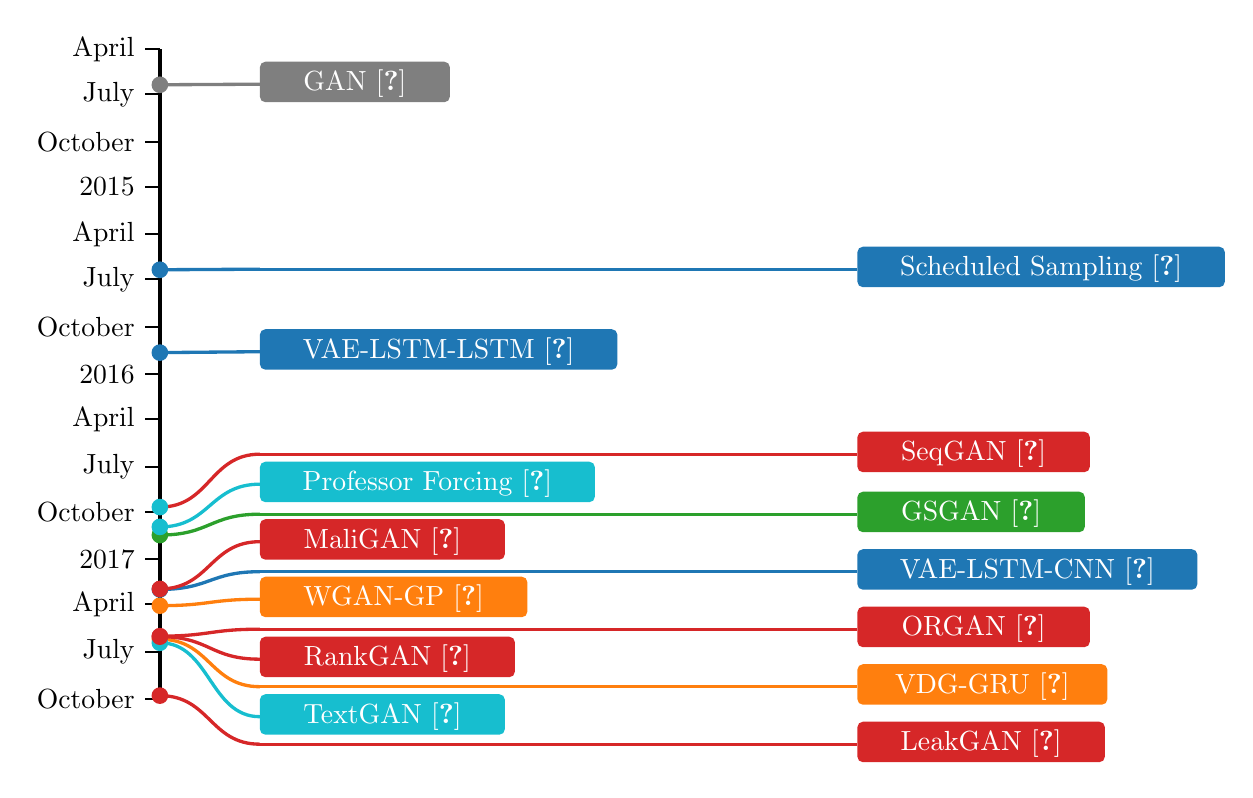
\begin{tikzpicture}[x=1bp,y=-1bp,scale=0.9]

% shift for the margin
\begin{scope}[shift={(20, 20)}]
% main layer
\begin{scope}[shift={(0, 0)}]
% axis
\begin{scope}
\draw[very thick] (0, 0) -- (0, 260);
\end{scope}

% axis layer
\begin{scope}
\begin{scope}[shift={(0, 0)}]
\draw[thick] (0, 0) -- (-6pt, 0)
node[anchor=east] {April};
\end{scope}
\begin{scope}[shift={(0, 18)}]
\draw[thick] (0, 0) -- (-6pt, 0)
node[anchor=east] {July};
\end{scope}
\begin{scope}[shift={(0, 37)}]
\draw[thick] (0, 0) -- (-6pt, 0)
node[anchor=east] {October};
\end{scope}
\begin{scope}[shift={(0, 55)}]
\draw[thick] (0, 0) -- (-6pt, 0)
node[anchor=east] {2015};
\end{scope}
\begin{scope}[shift={(0, 74)}]
\draw[thick] (0, 0) -- (-6pt, 0)
node[anchor=east] {April};
\end{scope}
\begin{scope}[shift={(0, 92)}]
\draw[thick] (0, 0) -- (-6pt, 0)
node[anchor=east] {July};
\end{scope}
\begin{scope}[shift={(0, 111)}]
\draw[thick] (0, 0) -- (-6pt, 0)
node[anchor=east] {October};
\end{scope}
\begin{scope}[shift={(0, 130)}]
\draw[thick] (0, 0) -- (-6pt, 0)
node[anchor=east] {2016};
\end{scope}
\begin{scope}[shift={(0, 148)}]
\draw[thick] (0, 0) -- (-6pt, 0)
node[anchor=east] {April};
\end{scope}
\begin{scope}[shift={(0, 167)}]
\draw[thick] (0, 0) -- (-6pt, 0)
node[anchor=east] {July};
\end{scope}
\begin{scope}[shift={(0, 185)}]
\draw[thick] (0, 0) -- (-6pt, 0)
node[anchor=east] {October};
\end{scope}
\begin{scope}[shift={(0, 204)}]
\draw[thick] (0, 0) -- (-6pt, 0)
node[anchor=east] {2017};
\end{scope}
\begin{scope}[shift={(0, 222)}]
\draw[thick] (0, 0) -- (-6pt, 0)
node[anchor=east] {April};
\end{scope}
\begin{scope}[shift={(0, 241)}]
\draw[thick] (0, 0) -- (-6pt, 0)
node[anchor=east] {July};
\end{scope}
\begin{scope}[shift={(0, 260)}]
\draw[thick] (0, 0) -- (-6pt, 0)
node[anchor=east] {October};
\end{scope}
\end{scope}

% link layer
\begin{scope}
\draw[color=linkColorA, very thick] (0, 14.229403524774408) .. controls
(20.0, 14.229403524774408) and (20.0, 14) .. (40, 14);
\draw[color=linkColorB, very thick] (0, 222.58852656611396) .. controls
(20.0, 222.58852656611396) and (20.0, 220) .. (40, 220);
\draw[color=linkColorC, very thick] (0, 236.00482131804412) .. controls
(20.0, 236.00482131804412) and (20.0, 255) .. (40, 255);
\draw[color=linkColorC, very thick] (40, 255) -- (239, 255);
\draw[color=linkColorC, very thick] (239, 255) .. controls
(259.0, 255) and (259.0, 255) .. (279, 255);
\draw[color=linkColorD, very thick] (0, 88.22230185360132) .. controls
(20.0, 88.22230185360132) and (20.0, 88) .. (40, 88);
\draw[color=linkColorD, very thick] (40, 88) -- (239, 88);
\draw[color=linkColorD, very thick] (239, 88) .. controls
(259.0, 88) and (259.0, 88) .. (279, 88);
\draw[color=linkColorE, very thick] (0, 121.36495423005505) .. controls
(20.0, 121.36495423005505) and (20.0, 121) .. (40, 121);
\draw[color=linkColorF, very thick] (0, 216.0921262664104) .. controls
(20.0, 216.0921262664104) and (20.0, 209) .. (40, 209);
\draw[color=linkColorF, very thick] (40, 209) -- (239, 209);
\draw[color=linkColorF, very thick] (239, 209) .. controls
(259.0, 209) and (259.0, 209) .. (279, 209);
\draw[color=linkColorG, very thick] (0, 194.34146659282666) .. controls
(20.0, 194.34146659282666) and (20.0, 186) .. (40, 186);
\draw[color=linkColorG, very thick] (40, 186) -- (239, 186);
\draw[color=linkColorG, very thick] (239, 186) .. controls
(259.0, 186) and (259.0, 186) .. (279, 186);
\draw[color=linkColorH, very thick] (0, 191.08903150144965) .. controls
(20.0, 191.08903150144965) and (20.0, 174) .. (40, 174);
\draw[color=linkColorI, very thick] (0, 237.42776167052153) .. controls
(20.0, 237.42776167052153) and (20.0, 267) .. (40, 267);
\draw[color=linkColorJ, very thick] (0, 183.15275108316774) .. controls
(20.0, 183.15275108316774) and (20.0, 162) .. (40, 162);
\draw[color=linkColorJ, very thick] (40, 162) -- (239, 162);
\draw[color=linkColorJ, very thick] (239, 162) .. controls
(259.0, 162) and (259.0, 162) .. (279, 162);
\draw[color=linkColorK, very thick] (0, 234.78515815877773) .. controls
(20.0, 234.78515815877773) and (20.0, 232) .. (40, 232);
\draw[color=linkColorK, very thick] (40, 232) -- (239, 232);
\draw[color=linkColorK, very thick] (239, 232) .. controls
(259.0, 232) and (259.0, 232) .. (279, 232);
\draw[color=linkColorL, very thick] (0, 234.98843535198878) .. controls
(20.0, 234.98843535198878) and (20.0, 244) .. (40, 244);
\draw[color=linkColorM, very thick] (0, 258.57705964752256) .. controls
(20.0, 258.57705964752256) and (20.0, 278) .. (40, 278);
\draw[color=linkColorM, very thick] (40, 278) -- (239, 278);
\draw[color=linkColorM, very thick] (239, 278) .. controls
(259.0, 278) and (259.0, 278) .. (279, 278);
\draw[color=linkColorN, very thick] (0, 215.88884907319934) .. controls
(20.0, 215.88884907319934) and (20.0, 197) .. (40, 197);
\end{scope}

% label layer
\begin{scope}
\begin{scope}[shift={(40, 5)}]
\fill[color=labelBgColorA, rounded corners=2pt]
(0, 0) rectangle (76, 16.2125) node[midway, yshift=-.75bp, anchor=center, text=labelTextColorA] {\strut \textA};
\end{scope}
\begin{scope}[shift={(40, 211)}]
\fill[color=labelBgColorB, rounded corners=2pt]
(0, 0) rectangle (107, 16.2125) node[midway, yshift=-.75bp, anchor=center, text=labelTextColorB] {\strut \textB};
\end{scope}
\begin{scope}[shift={(279, 246)}]
\fill[color=labelBgColorC, rounded corners=2pt]
(0, 0) rectangle (100, 16.2125) node[midway, yshift=-.75bp, anchor=center, text=labelTextColorC] {\strut \textC};
\end{scope}
\begin{scope}[shift={(279, 79)}]
\fill[color=labelBgColorD, rounded corners=2pt]
(0, 0) rectangle (147, 16.2125) node[midway, yshift=-.75bp, anchor=center, text=labelTextColorD] {\strut \textD};
\end{scope}
\begin{scope}[shift={(40, 112)}]
\fill[color=labelBgColorE, rounded corners=2pt]
(0, 0) rectangle (143, 16.2125) node[midway, yshift=-.75bp, anchor=center, text=labelTextColorE] {\strut \textE};
\end{scope}
\begin{scope}[shift={(279, 200)}]
\fill[color=labelBgColorF, rounded corners=2pt]
(0, 0) rectangle (136, 16.2125) node[midway, yshift=-.75bp, anchor=center, text=labelTextColorF] {\strut \textF};
\end{scope}
\begin{scope}[shift={(279, 177)}]
\fill[color=labelBgColorG, rounded corners=2pt]
(0, 0) rectangle (91, 16.2125) node[midway, yshift=-.75bp, anchor=center, text=labelTextColorG] {\strut \textG};
\end{scope}
\begin{scope}[shift={(40, 165)}]
\fill[color=labelBgColorH, rounded corners=2pt]
(0, 0) rectangle (134, 16.2125) node[midway, yshift=-.75bp, anchor=center, text=labelTextColorH] {\strut \textH};
\end{scope}
\begin{scope}[shift={(40, 258)}]
\fill[color=labelBgColorI, rounded corners=2pt]
(0, 0) rectangle (98, 16.2125) node[midway, yshift=-.75bp, anchor=center, text=labelTextColorI] {\strut \textI};
\end{scope}
\begin{scope}[shift={(279, 153)}]
\fill[color=labelBgColorJ, rounded corners=2pt]
(0, 0) rectangle (93, 16.2125) node[midway, yshift=-.75bp, anchor=center, text=labelTextColorJ] {\strut \textJ};
\end{scope}
\begin{scope}[shift={(279, 223)}]
\fill[color=labelBgColorK, rounded corners=2pt]
(0, 0) rectangle (93, 16.2125) node[midway, yshift=-.75bp, anchor=center, text=labelTextColorK] {\strut \textK};
\end{scope}
\begin{scope}[shift={(40, 235)}]
\fill[color=labelBgColorL, rounded corners=2pt]
(0, 0) rectangle (102, 16.2125) node[midway, yshift=-.75bp, anchor=center, text=labelTextColorL] {\strut \textL};
\end{scope}
\begin{scope}[shift={(279, 269)}]
\fill[color=labelBgColorM, rounded corners=2pt]
(0, 0) rectangle (99, 16.2125) node[midway, yshift=-.75bp, anchor=center, text=labelTextColorM] {\strut \textM};
\end{scope}
\begin{scope}[shift={(40, 188)}]
\fill[color=labelBgColorN, rounded corners=2pt]
(0, 0) rectangle (98, 16.2125) node[midway, yshift=-.75bp, anchor=center, text=labelTextColorN] {\strut \textN};
\end{scope}
\end{scope}

% dots
\begin{scope}
\draw node [circle, inner sep=0pt, minimum size=6bp, 
fill=dotColorA] at (0, 14.229404) {};
\draw node [circle, inner sep=0pt, minimum size=6bp, 
fill=dotColorB] at (0, 222.588527) {};
\draw node [circle, inner sep=0pt, minimum size=6bp, 
fill=dotColorC] at (0, 236.004821) {};
\draw node [circle, inner sep=0pt, minimum size=6bp, 
fill=dotColorD] at (0, 88.222302) {};
\draw node [circle, inner sep=0pt, minimum size=6bp, 
fill=dotColorE] at (0, 121.364954) {};
\draw node [circle, inner sep=0pt, minimum size=6bp, 
fill=dotColorF] at (0, 216.092126) {};
\draw node [circle, inner sep=0pt, minimum size=6bp, 
fill=dotColorG] at (0, 194.341467) {};
\draw node [circle, inner sep=0pt, minimum size=6bp, 
fill=dotColorH] at (0, 191.089032) {};
\draw node [circle, inner sep=0pt, minimum size=6bp, 
fill=dotColorI] at (0, 237.427762) {};
\draw node [circle, inner sep=0pt, minimum size=6bp, 
fill=dotColorJ] at (0, 183.152751) {};
\draw node [circle, inner sep=0pt, minimum size=6bp, 
fill=dotColorK] at (0, 234.785158) {};
\draw node [circle, inner sep=0pt, minimum size=6bp, 
fill=dotColorL] at (0, 234.988435) {};
\draw node [circle, inner sep=0pt, minimum size=6bp, 
fill=dotColorM] at (0, 258.577060) {};
\draw node [circle, inner sep=0pt, minimum size=6bp, 
fill=dotColorN] at (0, 215.888849) {};
\end{scope}

\end{scope}
\end{scope}
\end{tikzpicture}

\end{latin}
\hypersetup{citecolor=magenta}
%\hypersetup{citecolor=black}
\caption{نمایش زمانی روش‌های پیشین ارائه‌شده در حوزه‌ی تولید دنباله} 
\label{fig:chap2:timeline}
\end{figure}
